\documentclass[
  journal=pasa,
  manuscript=research-paper, %% or "review"
  year=2021,
  volume=37,
]{cup-journal}

\usepackage{microtype,siunitx,booktabs}

\DeclareRobustCommand{\VAN}[3]{#2}
\let\VANthebibliography\thebibliography
\def\thebibliography{\DeclareRobustCommand{\VAN}[3]{##3}\VANthebibliography}

%%%%% AUTHORS - PLACE YOUR OWN PACKAGES HERE %%%%%
\usepackage{graphicx}	% Including figure files
\usepackage{amsmath}	% Advanced maths commands
\usepackage{amssymb}	% Extra maths symbols
\usepackage{xspace}
\usepackage{upgreek}

%%%%%%%%%%%%%%%%%%%%%%%%%%%%%%%%%%%%%%%%%%%%%%%%%%

%%%%% AUTHORS - PLACE YOUR OWN COMMANDS HERE %%%%%

% COMMENTS
\newcommand{\SB}[1]{{\textcolor{purple}{#1}}}

% STELLAR LABELS
\newcommand{\Teff}{$T_\mathrm{eff}$\xspace}
\newcommand{\logg}{$\log g$\xspace}
\newcommand{\feh}{$\mathrm{[Fe/H]}$\xspace}
\newcommand{\numax}{$\nu_\mathrm{max}$\xspace}
\newcommand{\vmic}{$v_\mathrm{mic}$\xspace}
\newcommand{\vsini}{$v \sin i$\xspace}
\newcommand{\vrad}{$v_\mathrm{rad}$\xspace}

% NAMES
\newcommand{\TheCannon}{\textit{The Cannon}\xspace}
\newcommand{\sme}{\textsc{sme}\xspace}
\newcommand{\marcs}{\textsc{marcs}\xspace}
\newcommand{\Gaia}{\textit{Gaia}\xspace}
\newcommand{\TLF}{\Teff, \logg, and \feh}

% UNITS
\newcommand{\dex}{\,\mathrm{dex}}	% dex
\newcommand{\K}{\,\mathrm{K}}	% dex
\newcommand{\Msol}{\,\mathrm{M_\odot}} % Msol
\newcommand{\kpc}{\,\mathrm{kpc}}	% kpc
\newcommand{\mags}{\,\mathrm{mag}}	% mag
\newcommand{\yr}{\,\mathrm{yr}}	% Gyr
\newcommand{\Gyr}{\,\mathrm{Gyr}}	% Gyr
\newcommand{\eV}{\,\mathrm{eV}}	% eV
\newcommand{\Angstroem}{\,\text{\AA}}	% Angstroem
\newcommand{\kms}{\,\mathrm{km\,s^{-1}}}	% km/s
\newcommand{\kpckms}{\,\mathrm{kpc\,km\,s^{-1}}}	% kpc km/s
\newcommand{\kmkmss}{\,\mathrm{km^2\,s^{-2}}}	% km^2/s^2
\newcommand{\kmsMpc}{\,\mathrm{km\,s^{-1}\,Mpc^{-1}}}	% km/s/Mpc
\newcommand{\muHz}{\,\mathrm{\upmu Hz}} % micro Hz

\sisetup{detect-all,separate-uncertainty=true}

\title{The GALAH Survey: Data Release 4}

\author{S. Buder}
\affiliation{Research School of Astronomy \& Astrophysics, Australian National University, Canberra, ACT 2611, Australia}
\affiliation{ARC Centre of Excellence for All Sky Astrophysics in 3 Dimensions (ASTRO 3D), Australia}
\email[S. Buder]{sven.buder@anu.edu.au}

\author{The GALAH Collaboration}
% \alsoaffiliation{Joint first authors}

%\handlingeditor{Excellent E Editor}

\doi{10.1017/pasa.2020.32}

\received {dd Mmm YYYY}
\revised  {dd Mmm YYYY}
\accepted {dd Mmm YYYY}
\published{22 September 2020}

\keywords{
Surveys; the Galaxy; methods: observational; methods: data analysis; stars: fundamental parameters; stars: abundances} %% First letter not capped
% \jel{Q11; Q12; D81; M31}
% \msc{Q14; Q18; E21}
% \abbreviations{
%     BDHS: Bangladesh Demographic and Health Survey, 
%     IDA: Fe-deficiency anaemia, 
%     IFA: Fe-folic acid, 
%     MNP: multiple micronutrient powder, 
%     VAD: vitamin A deficiency
% }

\begin{document}

\begin{abstract}

For each spectrum, we find the best fitting model spectrum by employing a Bayesian framework that takes into account data as well as model uncertainties and can take non-spectroscopic information into account.

We fit all labels (elemental abundances and stellar parameters) simultaneously by using polynomial models created from synthetic spectra with randomly sampled labels for a restricted space in \Teff, \logg, and [Fe/H].

\end{abstract}

\section{INTRODUCTION}

\section{TARGET SELECTION AND OBSERVATION}

\section{REDUCTION} \label{sec:reduction}

Outcome of reduction pipeline:
\begin{table}
    \centering
    \caption{Data product 1: FITS files of reduced spectra}
    \label{tab:reduction_fits}
    \begin{tabular}{c|c}
    \hline \hline
    FITS Ext. & Description \\
    \hline
    Ext. 0 & Un-normalised signal~/~counts \\
    Ext. 1 & Normalised signal (by reduction pipeline) \\
    Ext. 2 & Relative uncertainty of signal \\
    Ext. 3 & Subtracted sky signal~/~counts \\
    Ext. 4 & Applied telluric correction \\
    Ext. 5 & Scattered light~/~counts \\
    Ext. 6 & Cross-talk \\
    Ext. 7 & Resolution profile~/~FWHM \\
    \hline
    \end{tabular}
\end{table}

\subsection{Line-spread function} \label{subsec:lsf}

$\texttt{fwhm}\,(\lambda)$, and $\texttt{b}$ reported for each CCD.

\begin{align}
    \exp \left(-0.693147 \vert 2x/\texttt{fwhm}\vert^\texttt{b}\right) \label{eq:lsf}
\end{align}

\newpage $\,$
\newpage

\section{ANALYSIS}

Our spectroscopic analyses uses a dedicated pipeline for GALAH spectra that implements the latest advancements in the modelling of stellar spectra taking into account for example 1D non-LTE effects and interpolating in the model space with computationally cheap algorithms. To reach agreement with non-spectroscopic information and solve possible degeneracies of the spectroscopic analysis, we run our pipeline in several ways in a Bayesian framework: we first only use spectroscopic information to estimate the most likely set of stellar labels (stellar parameters and abundances) to describe our data. In a second iteration, we also employ non-spectroscopic information as prior information to inform our analysis. We will denote posterior probability functions depending on the available/used observables:
\begin{align}
    P_\text{S} \quad &: \quad \text{only spectroscopy,} \\
    P_\text{SP} \quad &: \quad \text{also photo- and astrometry, and} \\
    P_\text{SPA} \quad &: \quad \text{also asteroseismology.}
\end{align}

We present the Bayesian framework to compute these functions in Sec.~\ref{subsec:bayes}. The link between these functions and our observables are several physical relations as well as models, most importantly the models that link stellar flux with stellar parameters and abundances. We describe this centerpiece of our spectroscopic analysis in Sec.~\ref{subsec:model_spectra} and how we adjust the observed spectra to best overcome imperfections based in the reduction on-the-fly in Sec.~\ref{subsec:adjustments_observation}. The machinery to find the best set of labels to describe our observables is described in Sec.~\ref{subsec:finding_best_labels}. The post-processing of outcomes on a spectrum-by-spectrum basis is described in Sec.~\ref{sec:post_processing} and the pipeline is validated in Sec.~\ref{sec:validation}.

\subsection{Bayesian framework} \label{subsec:bayes}

Previous versions of the GALAH pipelines used strict $\chi^2$ optimisation \citep{Buder2018} or treated non-spectroscopic information as ground-truth for computational reasons \citep{Buder2021}.

With the new modelling methodology available this data release, we are inspired by the previous works \citep[e.g.][]{Schoenrich2014, BailerJones2015, McMillan2018, Sharma2018} to simultaneously make a statistically more sound use of non-spectroscopic and prior information. 

We present the observables $\boldsymbol{y}$ and their uncertainties $\sigma_{\boldsymbol{y}}$ of our analysis in Sec.~\ref{subsubsec:observables}. In Sec.~\ref{subsubsec:labels}, we introduce the set of parameters, hereafter called labels $\boldsymbol{l}$ to generate models/predictions $\boldsymbol{y}_m(\boldsymbol{l})$ of the observables. Our analysis applies a simplified Bayesian statement
\begin{align}
    P( \boldsymbol{l} \vert \boldsymbol{y},\sigma_ {\boldsymbol{y}}) \propto P (\boldsymbol{y} \vert \boldsymbol{l}, \sigma_{\boldsymbol{y}}) P (\boldsymbol{l}).
\end{align}
Note here, that we ignore the normalisation constant $P(\boldsymbol{y}, \sigma_ {\boldsymbol{y}})$. We present our likelihood functions $P (\boldsymbol{y} \vert \boldsymbol{l}, \sigma_ {\boldsymbol{y}})$ in Sec.~\ref{subsubsec:likelihood} and the prior functions $P (\boldsymbol{l})$ in Sec.~\ref{subsubsec:prior}.

Because we run our pipeline with different sets of observables, we describe the different sets of probability functions $P( \boldsymbol{l} \vert \boldsymbol{y},\sigma_ {\boldsymbol{y}})$ in Sec.~\ref{subsubsec:probability}, which we will sample in order to create probability density functions (pdfs).

\subsubsection{Observables} \label{subsubsec:observables}

The industrial revolution in stellar surveys has allowed us to collect a plethora of spectroscpic ($f_\lambda~\pm~\sigma_{f_\lambda}$), photometric ($m_i~\pm~\sigma_{m_i}$), astrometric ($\varpi~\pm~\sigma_\varpi$), asteroseismic ($\nu_\text{max}~\pm~\sigma_{\nu_\text{max}}$ and $\delta_\nu~\pm~\sigma_{\delta_\nu}$)\SB{, and interferometric ($\Theta_\text{LD} \pm \sigma_{\Theta_\text{LD}}$)} measurements of stars. Each contribute ${\boldsymbol{y}_i} \pm \sigma_{\boldsymbol{y}_i}$ to our set of observables ${\boldsymbol{y}} \pm \sigma_{\boldsymbol{y}}$.

In our case, the GALAH reduction pipeline delivers $f_\lambda~\pm~\sigma_{f_\lambda}$ (see Sec.~\ref{sec:reduction}), but throughout our estimation of optimal stellar labels, we perform several adjustments to the data on-the-fly (see Sec.~\ref{subsec:adjustments_observation}).

We make use of photometric measurements from both the \Gaia mission \citep{Gaia-Collaboration2016}, specifically its eDR3 \citep{Brown2021}, and 2MASS \citep{Skrutskie2006}. The latter provides near infrared magnitudes $m_J$, $m_H$, and $m_{K_\text{S}}$. We use the three \Gaia bandpasses $m_G$, $m_{G_\text{BP}}$, and $m_{G_\text{RP}}$. We correct the $G$ flux and estimate the \Gaia magnitude uncertainties as described by \citet{Riello2021}. We use astrometric information $\varpi~\pm~\sigma_\varpi$ is provided by \Gaia eDR3 \citep{Lindegren2021a} and we apply the zero point correction to these measurements as described by \citep{Lindegren2021b}. Crossmatches to these catalogues are performed with \textsc{ADQL} queries on the \Gaia archive via \textsc{astroquery} by linking catalogue entries through the \texttt{source\_id} via the nearest neighbor matches provided by the \Gaia consortium on the \Gaia archive \citep[see][]{Marrese2017, Marrese2019}

We further crossmatch with the open cluster catalogue by \citet{CantatGaudin2020}\footnote{\SB{Update on this with \Gaia eDR3 as part of his 2021 paper?}} via \texttt{source\_id} and use their parallax estimates for stars with more than $70\%$ membership probabilities and more precise parallaxes. Similarly, we crossmatch with the globular cluster catalog by \citet{Vasiliev2021} via \texttt{source\_id} and use their parallax estimates for stars with more than $70\%$ membership probabilities and more precise parallaxes for the clusters NGC~104~/ 47~Tuc, NGC~288, NGC~362, NGC~1851, NGC~5139~/ $\omega$Cen, NGC~6362, NGC~6397, and NGC~7099~/ M~30.

Where available, we further use the asteroseismic parameters $\nu_\text{max}~\pm~\sigma_{\nu_\text{max}}$ and $\delta_\nu~\pm~\sigma_{\delta_\nu}$ by \SB{Zinn et al. (2021)}\footnote{\SB{Check this! What do we do if not all entries have uncertainties?}}.

\SB{For interferometric information ($\Theta_\text{LD} \pm \sigma_{\Theta_\text{LD}}$), we use a collection by \citet{Karovicova2020}, \citet{Karovicova2018}, and \citet{Heiter2015}, preferring the most recent values for each star.\footnote{\SB{Check this and also point to a catalog for people to trace back which one was used in the end... for each star. Also do not forget to cite the sources within \citet{Heiter2015}!}}}

\subsubsection{Model parameters (labels)} \label{subsubsec:labels}

To describe these observables (and their presumably Gaussian uncertainties), we can build models based on a specific set of parameters, hereafter called labels $\boldsymbol{l}$.

To predict a normalised stellar spectrum with flux $f \pm \sigma_f$, we need labels $\boldsymbol{l}_S$ that describe the photosphere of a star
\begin{align}
    \boldsymbol{l}_\text{S} \in \{
    T_\text{eff}, \log g, \mathrm{[Fe/H]}, \mathrm{[X/Fe]}, v_\mathrm{mic}, v \sin i, v_\text{rad}
    \}.
\end{align}

To describe photometric measurements of stars, typically reported in magnitudes $m_i \pm \sigma_{m_i}$ for filters $i$ with different bandpasses, we need a similar set of labels and information on the distance and extinction to properly scale a model star,
\begin{align}
    \boldsymbol{l}_\text{P} \in \{ T_\text{eff}, \log g, \mathrm{[Fe/H]}, \mathrm{[X/Fe]}, D_\varpi, A_V \}.
\end{align}
The distance will also allow us to predict measurements of parallaxes $\varpi \pm \sigma_\varpi$.

To describe the solar-like oscillations within low-mass stars, which can be transcribed to oscillation frequencies $\nu_\text{max} \pm \sigma_{\nu_\text{max}}$ \SB{and $\delta_\nu \pm \sigma_{\delta_\nu}$} via empirical asteroseismic scaling relations, we need \Teff, \logg, and masses,
\begin{align}
    \boldsymbol{l}_\text{A} \in \{ T_\text{eff}, \log g, \mathcal{M} \}.
\end{align}

Note that to avoid redundancy with labels in $\boldsymbol{l}_\text{S}$ and $\boldsymbol{l}_\text{P}$, we prefer the use of \logg over radius $\mathcal{R}$, which are fundamentally linked via $R = \sqrt{\mathrm{G} \mathcal{M} g^{-1}}$.

\subsubsection{Likelihood functions} \label{subsubsec:likelihood}

Assuming that the uncertainties $\sigma_{\boldsymbol{y}_i}$ of our observables $\boldsymbol{x}$ are Gaussian, we can define a likelihood for each individual observable ${\boldsymbol{y}_i}$ with a model prediction $\boldsymbol{y}_{i,m} (\boldsymbol{l})$
\begin{align}
    G({\boldsymbol{y}_i}, {\boldsymbol{y}_{i,m}} (\boldsymbol{l}), \sigma_y) = \frac{1}{\sqrt{2\pi} \sigma_{\boldsymbol{y}_i}} \exp \left( -  \frac{\left({\boldsymbol{y}_i} - {\boldsymbol{y}_{i,m}} (\boldsymbol{l})\right)^2}{2 \sigma_{\boldsymbol{y}_i}^2}\right)
\end{align}
or in logarithmic form
\begin{align}
    \ln G({\boldsymbol{y}_i}, {\boldsymbol{y}_{i,m}} (\boldsymbol{l}), \sigma_{\boldsymbol{y}_i}) = - \frac{1}{2} \left( \ln (2 \pi \sigma_y) + \frac{\left({\boldsymbol{y}_i} - {\boldsymbol{y}_{i,m}} (\boldsymbol{l})\right)^2}{\sigma_{\boldsymbol{y}_i}^2} \right).
\end{align}

We describe how we actually create model spectra ${\boldsymbol{y}_{i,m}} (\boldsymbol{l}_S)$ in Sec.~\ref{subsec:model_spectra}. To calculate the total spectroscopic logarithmic likelihood, we sum the likelihood of each pixel $i=\lambda$ over all $n$ pixels
\begin{align} \label{eq:likelihood_spectroscopic}
    \ln P_S ({\boldsymbol{f}} \vert {\boldsymbol{l}_S}, \sigma_{\boldsymbol{f}}) = \sum_\lambda^n \ln G({\boldsymbol{f}_\lambda}, {\boldsymbol{f}_{\lambda,m}} (\boldsymbol{l}_S), \sigma_{\boldsymbol{f}_\lambda}).
\end{align}

Predicting photometric and astrometric observables, that is magnitudes and parallaxes, is an interconnected task. While the parallax $\varpi$ can be easily predicted by the inverse of the distance $D_\varpi$,
\begin{align}
    \varpi = \frac{1000\,\mathrm{mas}}{D_\varpi~/~\mathrm{pc}},
\end{align}
magnitudes $m_i$ of certain photometric filters $i$ need to be predicted on an absolute scale $M_i$ and then scaled with distance $D_\varpi$ and a possible extinction within the filter $A_i$
\begin{align} \label{eq:magnitudes}
    m_i = M_i + 5 \log\frac{D_\varpi}{10\,\mathrm{pc}} + A_i.
\end{align}
We use the isochrone tables provided by the stellar evolutionary \textsc{parsec} \citep[v. 1.2][]{Bressan2012, Tang2014, Chen2014, Chen2015} and \textsc{colibri} \citep[S\_37, S\_35 and PR16][]{Marigo2013, Rosenfield2016, Marigo2017, Pastorelli2019, Pastorelli2020} to predict magnitudes in the photometric systems of 2MASS \citep{Cohen2003} and \Gaia eDR3 \citep{Riello2021}. We use version 3.5 of the interface \textsc{cmd}\footnote{\url{http://stev.oapd.inaf.it/cmd}} to download isochrone grids with a fine sampling of $\log (\tau~/~\mathrm{Gyr}) = 6.19..(0.01)..10.18$ for age as well as a broad and fine sampling of $\mathrm{[M/H]} = -2.75..(0.25)..-0.75\,\mathrm{dex}$ and $\mathrm{[M/H]} = -0.60..(0.10)..0.70\,\mathrm{dex}$, respectively. We adopt default values of \textsc{cmd} version 3.5, except for the initial mass function, for which we use the exponential function (see also Eq.~\ref{eq:chabrier}) by \citet{Chabrier2001}. For the extinction in the individual filters, we adopt the \textsc{cmd} values of $A_{G}/A_V = 0.83627$,
$A_{G_\text{BP}}/A_V = 1.08337$,
$A_{G_\text{RP}}/A_V = 0.63439$
$A_{J}/A_V = 0.28665$,
$A_{H}/A_V = 0.18082$, and
$A_{K_\text{S}}/A_V = 0.11675$.
% $A_{W_1}/A_V = 0.05688$,
% $A_{W_2}/A_V = 0.03427$,
% $A_{W_3}/A_V = 0.00707$, and
% $A_{W_4}/A_V = 0.00274$
We train a \textsc{sklearn} \textsc{cKDtree} on the isochrone grid points of \Teff, \logg, \SB{[M/H]}\footnote{\SB{Currently we use [M/H] = [Fe/H], rather than [M/H] = $f(\mathrm{[Fe/H]},\mathrm{[X/Fe]})$!}}. We can then query it with the specific labels to get a prediction of mass $\mathcal{M}$ and age $\tau$ as well as absolute magnitudes $M_i$ (see Eq.~\ref{eq:magnitudes}) for $i \in \{G, G_\text{BP}, G_\text{RP}, J, H, K_\text{S}\}$.

Thanks to the GALAH selection function, all GALAH targets have both astrometric and asteroseismic information and we can thus treat this information always together. This allows us to define a photoastrometric logarithmic likelihood functions
\begin{align} \label{eq:likelihood_photoastrometric}
    \ln P_P (\varpi, {\boldsymbol{m}} \vert {\boldsymbol{l}_P}, \sigma_\varpi, \sigma_{\boldsymbol{m}} ) = 
    \sum_{i \in {\varpi,{\boldsymbol{m}}}}
    \ln G({\boldsymbol{y}_i}, {\boldsymbol{y}_{i,m}} (\boldsymbol{l}_P), \sigma_{\boldsymbol{y}_i}).
\end{align}

Asteroseismic observables are typically predicted via empirical scaling relations by \citet{Kjeldsen1995}. In our case, we use labels ${\boldsymbol{l}_A}$ to predict the frequency of maximum power
\begin{align}
    % \nu_{\text{max},m} = \frac{\mathcal{M}~/~\mathrm{M_\odot}}{\left(\mathcal{R}~/~\mathrm{R_\odot}\right)^2} \sqrt{\frac{T_\text{eff}}{5772\,\mathrm{K}}} \times 3090\muHz,
    \nu_{\text{max},m} = \frac{10^{\log g}}{10^{4.438}\,\mathrm{cm\,s^{-2}}} \sqrt{\frac{T_\text{eff}}{5772\,\mathrm{K}}} \times 3090\muHz
\end{align}
and the large frequency separation
\begin{align}
    %\delta_{\nu,m} = \left( \mathcal{M}~/~\mathrm{M_\odot} \right)^{\frac{1}{2}} \left( \mathcal{R}~/~\mathrm{R_\odot} \right)^{-\frac{3}{2}} \times 134.9\muHz.
    \delta_{\nu,m} = \left( \frac{\mathcal{M}}{\mathrm{M_\odot}} \right)^{\frac{-1}{4}} \left( \frac{10^{4.438}\,\mathrm{cm\,s^{-2}}}{10^{\log g}} \right)^{-\frac{3}{4}} \times 134.9\muHz.
\end{align}
In these, we incorporate the Solar values $\nu_{\text{max},\odot} = 3090\muHz$, $\delta_{\nu,\odot} = 134.9\muHz$ and $T_{\mathrm{eff},\odot} = 5772\,\mathrm{K}$ as constants. This allows us to define a logarithmic likelihood function\footnote{\SB{Note: We are currently only using $\nu_\text{max}$, because some $\delta_\nu$ are missing, and some $\sigma_{\delta_\nu}$ are 0.}}
\begin{align} \label{eq:likelihood_asteroseismic}
    \ln P_A (\nu_\text{max}, \delta_\nu \vert {\boldsymbol{l}_A}, \sigma_{\nu_\text{max}}, \sigma_{\delta_\nu}) = 
    \sum_{i \in {\nu_\text{max},\delta_\nu}}
    \ln G({\boldsymbol{y}_i}, {\boldsymbol{y}_{i,m}} (\boldsymbol{l}_A), \sigma_{\boldsymbol{y}_i}).
\end{align}

\SB{We predict the angular diameters $\Theta_\text{LD}$ based on the mass, surface gravity and distance via
\begin{align}
    \Theta_\text{LD} = 2 \arctan \left( \sqrt{\frac{\mathrm{G} \mathcal{M}}{10^{\log g}}} \frac{1}{D_\varpi} \right).
\end{align}}

\SB{Available but not used: infrared photometry $W_1$ - $W_4$ from WISE \citep{Cutri2013}}

\subsubsection{Prior functions} \label{subsubsec:prior}

We formulate a series of priors and apply the relevant ones depending on the set of input information.

As our model spectra are restricted to the \marcs model grid (see red points in Fig.~\ref{fig:teff_logg_grid_coverage}), we will impose the convex hull as prior on the main stellar parameters \Teff, \logg, and \feh to be within the \marcs atmosphere model grid \citep{Gustafsson2008}, used to create model spectra (see Sec.~\ref{subsec:model_spectra}).
\begin{align}
    P(T_\mathrm{eff}, \log g, \mathrm{[Fe/H]}) = \begin{cases}
    1 \quad \text{within \marcs grid} \\
    0 \quad \text{otherwise} \\
    \end{cases}
\end{align}
We restrict to the $T_\text{eff} \geq 3100 - 100\K$ for computational reasons as well as $\mathrm{[Fe/H]} \geq -3 - 1\dex$ and because we do expect only a handful of stars below this range. The maximum extend of this hull is then up to $3000 \leq T_\text{eff}~/~\mathrm{K} \leq 8000$, $-0.5 \leq \log (g~/~\mathrm{cm\,s^{-2}}) \leq 5.5$, and $-4 \leq \mathrm{[Fe/H]}~/~\mathrm{dex} \leq 1$.

\begin{align}
    P(v_\text{mic}) &= \begin{cases}
    1 \quad v_\text{mic} > 0.0\kms \\
    0 \quad \text{otherwise} \\
    \end{cases} \\
    P(v \sin i) &= \begin{cases}
    1 \quad v \sin i > 0.0\kms \\
    0 \quad \text{otherwise} \\
    \end{cases} \\
    P(\nu_\text{max}) &= \begin{cases}
    1 \quad \nu_\text{max} > 0\muHz \\
    0 \quad \text{otherwise} \\
    \end{cases} \\
    P(D_\varpi) &= \begin{cases}
    1 \quad D_\varpi \geq 0\kpc \\
    0 \quad \text{otherwise} \\
    \end{cases} \\
    P(A_V) &= \begin{cases}
    1 \quad A_V \geq 0\mags \\
    0 \quad \text{otherwise} \\
    \end{cases}
\end{align}

\SB{Mass is not a stellar label at the moment, but interpolated from isochrones. If we include it to be sampled and used both for isochrones and $\delta_\nu$, shall we impose a flat mass prior between 0.1 and $4.0\Msol$ or a mass prior à la \citet{Chabrier2001}, as done in \citet{Sharma2018}?
\begin{align} \label{eq:chabrier}
    P(\mathcal{M}) = 22.8978 \exp \left[ - \left(\frac{716.4\Msol}{\mathcal{M}}\right)^{0.25} \right] \left( \frac{\mathcal{M}}{\Msol} \right)^{-3.3}
\end{align}
}

With this, we can formulate a prior function $P_s (\boldsymbol{l}_S)$ for the purely spectroscopic analysis:
\begin{align}
    P_S ( \boldsymbol{l}_S ) = P(T_\text{eff}, \log g, \mathrm{[Fe/H]}) P(v_\text{mic}) P(v\sin i)
\end{align}

If we also fit photo-astrometric information, we further impose a prior
\begin{align}
    P_{SP} ( \boldsymbol{l}_S ) = P_s ( \boldsymbol{l}_S ) P(D_\varpi) P (A_V)
\end{align}

If we also fit asteroseismic information, we further impose a prior
\begin{align}
    P_{SPA} ( \boldsymbol{l}_S ) = P_S ( \boldsymbol{l}_S ) P(\nu_\text{max}) P(\delta_\nu) P(D_\varpi) P (A_V)
\end{align}

\subsubsection{Posterior probability functions} \label{subsubsec:probability}

With our likelihood and prior functions, we can find combinations of different posterior probability functions.

If we do only take into account spectroscopic information, we will use the posterior
\begin{align} \label{eq:posterior_s}
    P_S = P ( \boldsymbol{l}_S \vert {\boldsymbol{f}}, \sigma_{\boldsymbol{f}} ) = P ( {\boldsymbol{f}} \vert \boldsymbol{l}_S, \sigma_{\boldsymbol{f}} ) \times P_S ( \boldsymbol{l}_S ).
\end{align}

If we take both spectroscopic and photoastrometric information into account, we will use
\begin{align}\label{eq:posterior_sp}
    P_{SP} = P ( \boldsymbol{l}_{SP} \vert {\boldsymbol{f}}, {\boldsymbol{m}}, \varpi, \sigma_{\boldsymbol{f}} , \sigma_{\boldsymbol{m}}, \sigma_\varpi) = \notag\\
    P ( {\boldsymbol{f}}, {\boldsymbol{m}}, \varpi \vert \sigma_{f}, \sigma_{\boldsymbol{m}}, \sigma_\varpi, \boldsymbol{l}_{SP} ) ~ P_{SP} ( \boldsymbol{l}_{SP} ).
\end{align}

If we additionally also use available asteroseismic measurements, we use
\begin{align}\label{eq:posterior_spa}
    P_{SPA} = P ( \boldsymbol{l}_{SPA} \vert {\boldsymbol{f}}, {\boldsymbol{m}}, \varpi, {\nu_\text{max}}, {\delta_\nu}, \sigma_{\boldsymbol{f}} , \sigma_{\boldsymbol{m}}, \sigma_\varpi, \sigma_{\nu_\text{max}}, \sigma_{\delta_\nu}) = \notag\\
    P ( {\boldsymbol{f}}, {\boldsymbol{m}}, \varpi, {\nu_\text{max}}, {\delta_\nu} \vert \sigma_{f}, \sigma_{\boldsymbol{m}}, \sigma_\varpi, \sigma_{\nu_\text{max}}, \sigma_{\delta_\nu}, \boldsymbol{l}_{SP} ) ~ P_{SPA} ( \boldsymbol{l}_{SPA}).
\end{align}

\subsection{Creating model spectra} \label{subsec:model_spectra}

In our endeavour to push the limits even further, we are advancing our analysis to fit all 30 elemental abundances and stellar parameters across the full GALAH wavelength range simultaneously with the appropriate model spectra.

To make this computationally feasible, we follow an idea reported by \citet{Rix2016} and create polynomial models for smaller parts of the parameters space from only a limited number of ab initio models \citep[see also][]{Ting2016b}. Our ab initio models are calculated with Spectroscopy Made Easy \citep[\textsc{sme}][]{Valenti1996,Piskunov2017} for the whole wavelength range and all visible atomic and molecular lines for random selections of elemental abundances and stellar parameters within the range of \textsc{marcs} atmospheres \citep{Gustafsson2008}. We then select subsets of these spectra within a restricted space of the three main spectroscopic parameters \Teff, \logg, and [Fe/H]. This idea is comparable to selecting solar twin spectra when analysing the Sun \citep[see e.g.][who applied this idea with tremendous success in the opposite direction]{Nissen2015}. For each subset, we train a quadratic model that correlates stellar flux and labels (stellar parameters and abundances) in the framework of \textit{The Cannon} \citep{Ness2015, Casey2016}. With these models, we can then create model spectra with all lines over the whole wavelength range for any combination of element abundances within this restricted parameter space within less than a second (compared to minutes or hours for physics-driven syntheses). 

In order to confront these model spectra with the GALAH observations, we downgrade the model spectra on-the-fly with the available line-spread functions of each observation (see Sec.~\ref{subsec:lsf}).

\subsubsection{Grid of synthetic spectra} \label{subsubsec:spectrum_grid}

To achieve a self-consistent grid of synthetic spectra, we compute significantly over-sampled synthetic spectra at 10- times higher then the typical GALAH resolution with \sme.

We select small parts, that is 3D bins of the parameter space of \Teff, \logg, and \feh. For each of these parameters, we loop through the \marcs grid and compute randomly selected spectra within $\pm 1$ grid points in \Teff (with either $\pm 250$ or $\pm 100\K$), \logg ($\pm 0.5\dex$), and \feh ($\pm 1.0$, $\pm 0.5$ or $\pm 0.25\dex $).

We explain the sampling of parameters and abundances in an exemplary way for the 3D bin centred on $T_\text{eff} = 5750\pm250\K$, $\log g = 4.5\pm0.5\dex$ and $\mathrm{[Fe/H]} = 0.0\pm0.25\dex$ (see blue box in Fig.~\ref{fig:teff_logg_grid_coverage}).

For each synthetic spectrum to be computed within this 3D bin, the stellar parameters (\Teff, \logg, \feh, \vmic) and elemental abundances [X/Fe] of all 30 elements are randomly sampled within reasonable limits (see Eqs.~\ref{eq:sampling_teff}-\ref{eq:sampling_xfe}) and fed into \sme to create self-consistent synthetic spectra over the full wavelength range for \marcs atmospheres:
\begin{align} 
    T_\text{eff}~/~\K &\in {5500..5750..6000} \\ \label{eq:sampling_teff}
    \log g~/~\dex &\in {4.0..4.5..5.0} \\
    \mathrm{[Fe/H]}~/~\dex &\in {-0.25..0.0..0.25} \\
    v_\text{mic}~/~\kms &\in {0.5..1.5..4.0} \\
    v \sin i~/~\kms &= 0\text{, but see Eq.~\ref{eq:vsini}} \\
    \mathrm{A(Li)} &\in \begin{cases} {-0.55..2.75..3.76} \\ {-1.0..5.0}  \end{cases} \\
    \mathrm{[O/Fe]}, \mathrm{[Y/Fe]}, \mathrm{[Ba/Fe]} &\in \begin{cases} {-2.0..0.0..2.0} \\ {-1.0..0.0..1.0}  \end{cases} \\
    \mathrm{[X/Fe]} &\in \begin{cases} {-1.0..0.0..1.0} \\ {-0.5..0.0..0.5} \label{eq:sampling_xfe} \end{cases}
\end{align}

\begin{figure}[hbt!]
 \centering
 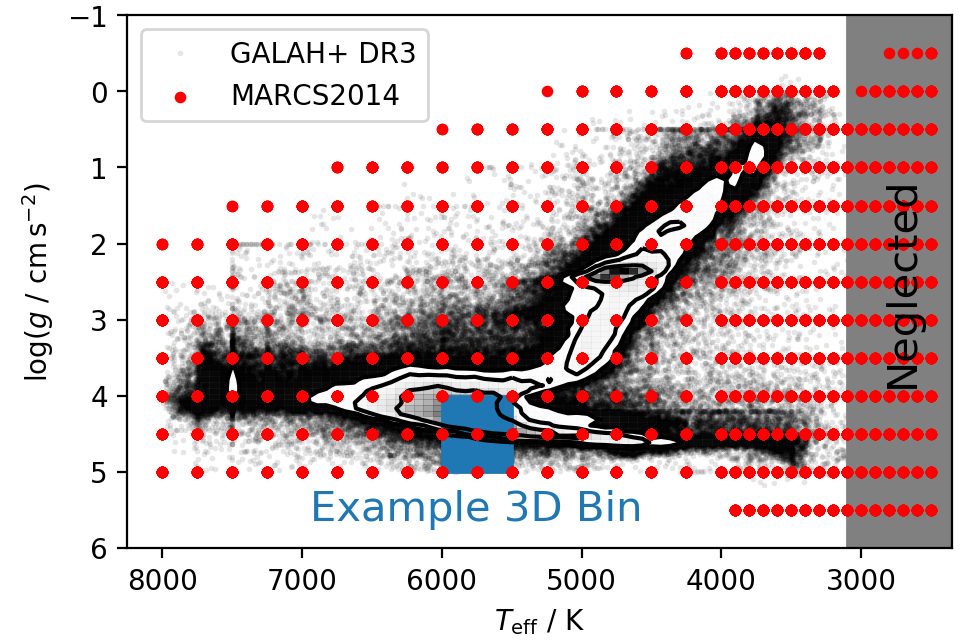
\includegraphics[width=\textwidth]{figures/teff_logg_grid_coverage.png}
 \caption{Coverage in \Teff and \logg of MARCS2014 grid (red) and GALAH DR3 (black, including density countour). Shown is also an example of one of the 3D bins used to create models with \TheCannon. MARCS grid points \Teff$ < 3100\K$ or \feh$<-3\dex$ are neglected throughout GALAH DR4.}
 \label{fig:teff_logg_grid_coverage}
\end{figure}

For each spectrum, we first run a test on all available lines in the GALAH linelist, which is adapted from \citet{Heiter2021} and includes small changes to correct wrong $\log gf$ values for few lines within the GALAH wavelength range. We keep all atomic lines for the final synthesis and restrict the molecular lines to those with \textsc{sme}.depth above 0.001.

Spectra are computed at a resolution of $R = 1,000,000$ on a fine wavelength grid with 60,819 pixels spread over the extended wavelengths $4675.1- 4949.9$, $5624.1-5900.9$, $6424.1-6775.9$, and $7549.1-7925.9 \Angstroem$. We note that these extend significantly beyond the actual GALAH wavelength range.

We use 1D \marcs atmospheres from the \marcs grid \citep[][version 2014]{Gustafsson2008}, and interpolate them for combinations of \Teff, \logg, and \feh. We use grids of non-LTE departure coefficients by \citet{Amarsi2020} for H, Li, C, N, O, Na, Mg, Al, Si, K, Ca, Mn, and Ba. For all, except C, we use grids that include background scattering.

To be able to test that the flux-label correlations found by our subsequent polynomial interpolation are limited to reasonable wavelength ranges, we also calculate one spectrum that is exactly in the middle of the parameter range and additional spectra, where we increase the value of one label at a time (e.g. increase [O/Fe] by $1\dex$) to test the response in the synthetic spectrum.

To save computational power, we compute synthetic spectra with no rotational or macroturbulence broadening ($v_\text{mac} = v\sin i = 0\kms$), but save the model continuum flux (\texttt{sme.cmod}) and the specific intensities (\texttt{sme.sint}) as a function of the equal-area midpoints of each equal-area annulus $\mu$ (see Fig.~\ref{fig:sme_mu_output}). These can be integrated after-the fact to sample different \vsini values for the polynomical models (see Sec.~\ref{subsubsec:polynomials}).

\begin{figure*}[hbt!]
 \centering
 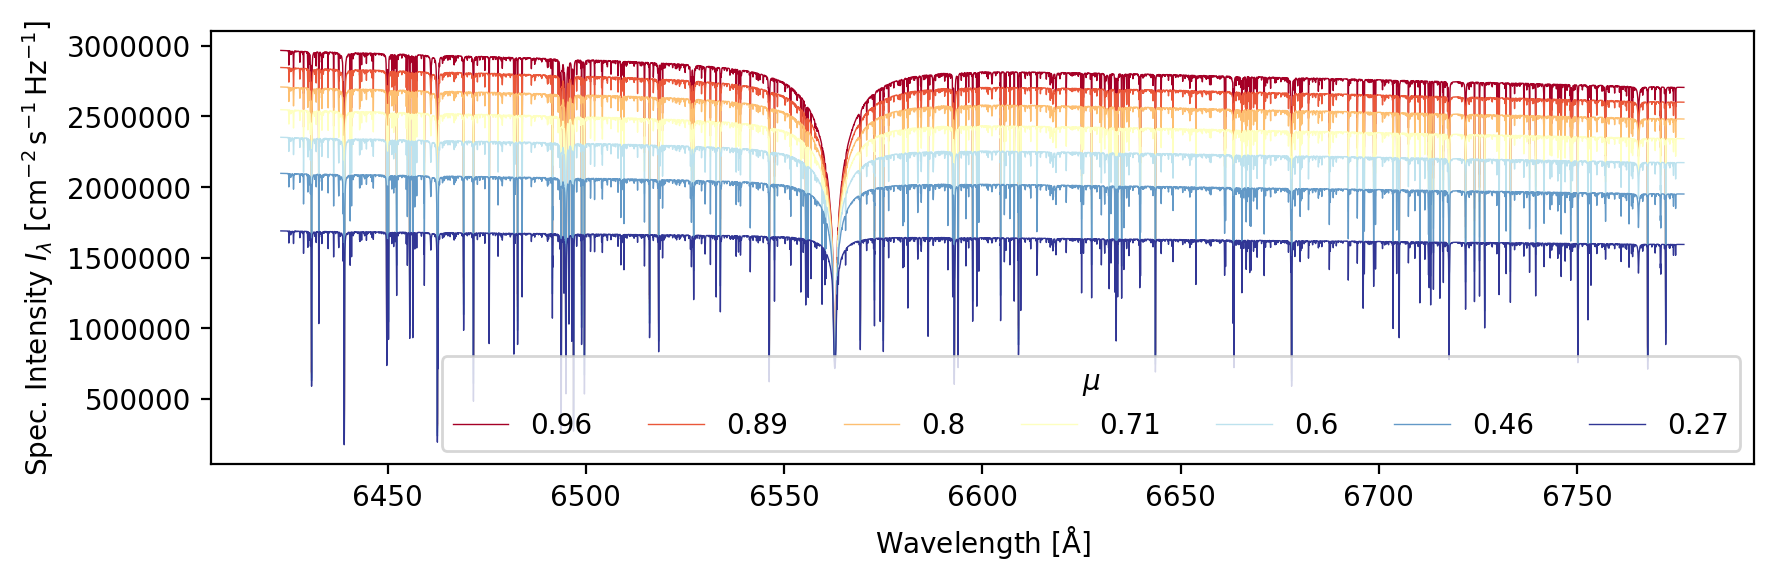
\includegraphics[width=\textwidth]{figures/solar_twin_specific_intensity.png}
 \caption{Example output of \sme for a solar spectrum in HERMES CCD3 (around the Balmer $\mathrm{H}_\alpha$ line). Shown are the the specific intensities (\texttt{sme.sint}) as a function of the equal-area midpoints of each equal-area annulus $\mu$.}
 \label{fig:sme_mu_output}
\end{figure*}

Our synthetic grid explicitly includes C and N abundances. C was previously included in the analysis of GALAH DR3, but limited to the atomic C line. The analysis thus neglected the molecular absorption features of $\mathrm{C_2}$ and CN at the beginning of CCD1 and end of CCD4, respectively. With the new self-consistent grid, we can however include these features, as they hold valuable information for both C and N, as well as several other features through the molecular equilibrium in stars \citep[see e.g.][]{Ting2018}.

\subsubsection{Polynomial models for a subset} \label{subsubsec:polynomials}

\begin{figure*}[hbt!]
 \centering
 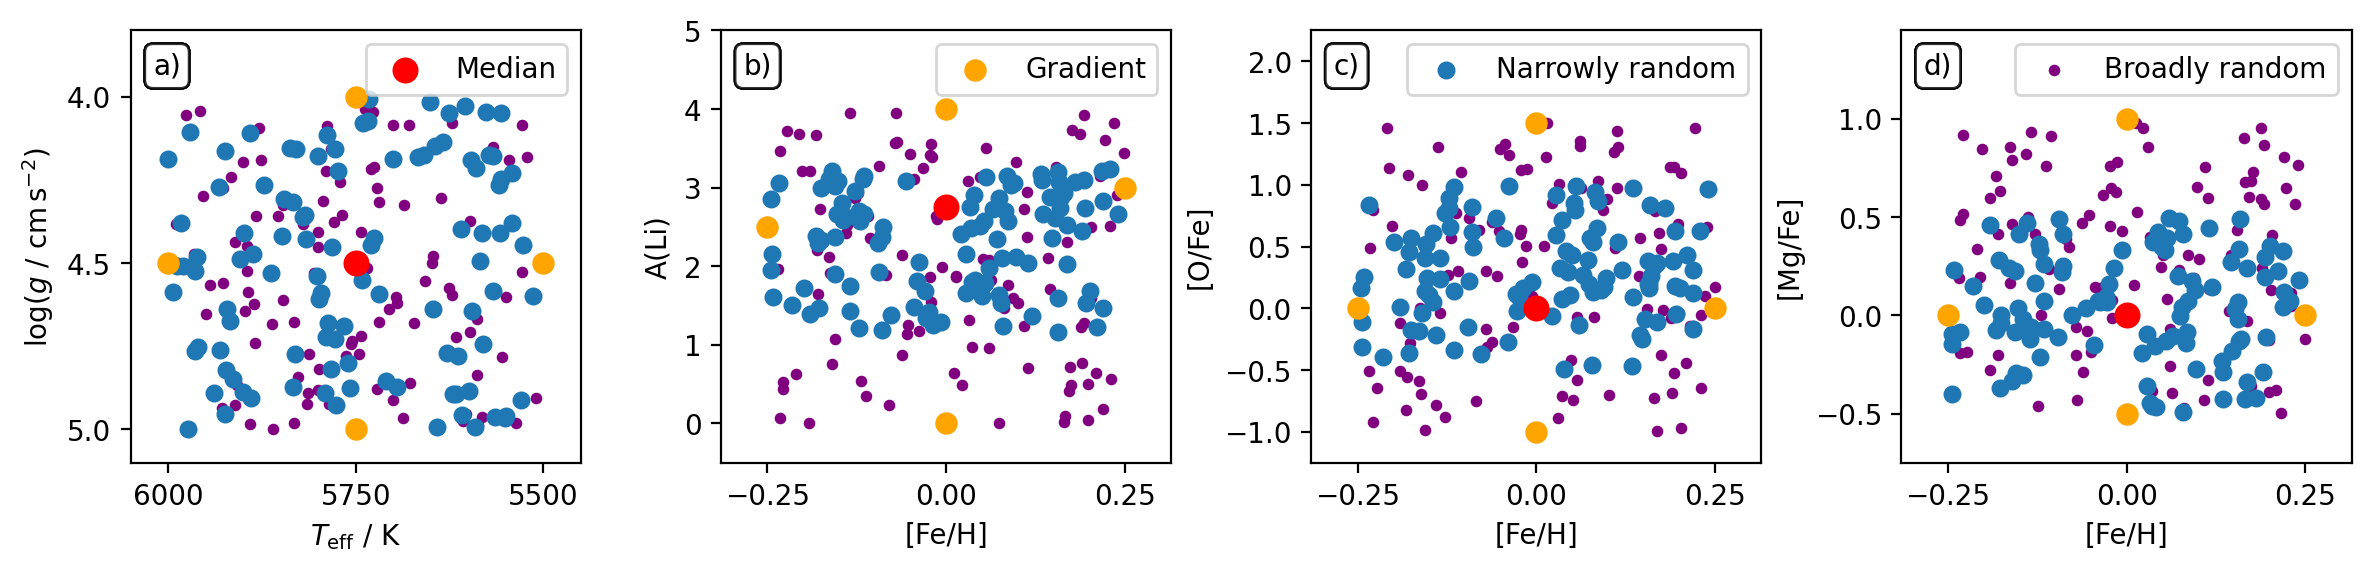
\includegraphics[width=\textwidth]{figures/example_3d_bin_sample.png}
 \caption{\textbf{Coverage of stellar parameters and abundances for one of the 3D bins.} Shown is the example of the solar 3D bin ($T_\mathrm{eff}~/~\mathrm{K} = 5750$, $\log (g~/~\mathrm{cm\,s^{-2}}) = 4.5$, $\mathrm{[Fe/H]}~/~\mathrm{dex} = 0.0$). \textbf{Panel a):} \Teff and \logg, \textbf{Panel b):} [Fe/H] vs. [Li/Fe], \textbf{Panel c):} [Fe/H] vs. [O/Fe], \textbf{Panel d):} [Fe/H] vs. [Mg/Fe]. While \Teff, \logg, and \feh are sampled randomly within the 3D bin, the abundances are sampled both narrowly (blue) and broadly (purple) within limits as described in the text. Red point indicate the median spectrum and orange points the adjusted spectra to test the gradient change of spectra with individual label.}
 \label{fig:cannon_interpolation}
\end{figure*}

We are training 2499 models for the individual but overlapping 3D bins in \Teff, \logg, and \feh (see again Fig.~\ref{fig:teff_logg_grid_coverage} as example).

At this stage, we explicitly include the broadening of spectra because of rotation (\vsini) and sample each of the synthetic spectra over a range of
\begin{align} \label{eq:vsini}
    v \sin i~/~\kms \in \{ 1.5, 3.0, 6.0, 9.0, 12.0, 24.0\}.
\end{align}

The decision for these values was made based on the distribution of \vsini ($7.2_{-1.6}^{4.9}\kms$ with 90\% between 4.7 and $29.0\kms$) in GALAH+ DR3 and comparison with the grid values used by APOGEE DR16 \citep{Joensson2020}.

Our interpolation method does not care about the stellar physics behind the correlation of stellar flux and labels. We thus introduce an intermediate step to verify that the found correlations are at least limited to the wavelength regions where we would expect a reaction to the specific label. This technique is called censoring \citep{Casey2016} or masking \citep{Buder2018}. For our analysis, we explicitly have included perturbations for one label at a time to a median spectrum of the grid. Comparing the median with each of the perturbed spectra at the highest rotational broadening ($v \sin i = 24.0\kms$) allows us to assess which pixels of the synthetic spectra change and only allow the polynomial fitting to find non-zero coefficients for the particular label for exactly these pixels. The idea here is, that coefficients related to Li should for example only be allowed to be non-zero where the spectrum also responds to Li (like the Li line).

\begin{table}
    \centering
    \caption{Example of mask estimation for \textit{The Cannon} model creation. Listed are percentages of the spectrum that respond to an in-/decrease of each label above 0.001 and 0.0001 of the normalised flux.}
    \label{tab:cannon_mask_percentage}
    \begin{tabular}{cccc}
    \hline \hline
    Label &  Label change & $\vert \Delta f \vert > 0.001~/~\%$ & $\vert \Delta f \vert > 0.0001~/~\%$ \\
    \hline
    $T_\mathrm{eff}~/~\mathrm{K}$ & $\pm$250.0 & 99.2 & 85.1 \
    $\log (g~/~\mathrm{cm\,s^{-2}})$ & $\pm$0.5 & 93.3 & 54.2 \
    [Fe/H] & $\pm$0.25 & 99.6 & 95.6 \
    $v_\mathrm{mic}~/~\mathrm{km\,s^{-1}}$ & $\pm$1.0 & 61.6 & 39.8 \
    [Li/Fe] & $\pm$2.25 & 1.9 & 0.6 \
    [C/Fe] & $\pm$1.0 & 99.2 & 95.1 \
    [N/Fe] & $\pm$1.0 & 98.3 & 87.7 \
    [O/Fe] & $\pm$2.0 & 98.6 & 82.9 \
    [Na/Fe] & $\pm$1.0 & 74.0 & 30.1 \
    [Mg/Fe] & $\pm$1.0 & 98.8 & 82.2 \
    [Al/Fe] & $\pm$1.0 & 78.2 & 34.8 \
    [Si/Fe] & $\pm$1.0 & 97.6 & 73.7 \
    [K/Fe] & $\pm$1.0 & 29.1 & 2.1 \
    [Ca/Fe] & $\pm$1.0 & 83.8 & 44.8 \
    [Sc/Fe] & $\pm$1.0 & 10.6 & 4.8 \
    [Ti/Fe] & $\pm$1.0 & 63.5 & 32.9 \
    [V/Fe] & $\pm$1.0 & 35.5 & 18.8 \
    [Cr/Fe] & $\pm$1.0 & 72.4 & 38.0 \
    [Mn/Fe] & $\pm$1.0 & 48.0 & 13.7 \
    [Co/Fe] & $\pm$1.0 & 39.7 & 19.9 \
    [Ni/Fe] & $\pm$1.0 & 79.9 & 43.4 \
    [Cu/Fe] & $\pm$1.0 & 2.7 & 0.8 \
    [Zn/Fe] & $\pm$1.0 & 3.2 & 0.8 \
    [Rb/Fe] & $\pm$1.0 & 0.3 & 0.1 \
    [Sr/Fe] & $\pm$1.0 & 2.1 & 1.5 \
    [Y/Fe] & $\pm$2.0 & 20.8 & 9.3 \
    [Zr/Fe] & $\pm$1.0 & 8.5 & 3.3 \
    [Mo/Fe] & $\pm$1.0 & 4.0 & 0.9 \
    [Ru/Fe] & $\pm$1.0 & 3.2 & 1.0 \
    [Ba/Fe] & $\pm$2.0 & 13.8 & 6.2 \
    [La/Fe] & $\pm$1.0 & 4.5 & 3.3 \
    [Ce/Fe] & $\pm$1.0 & 51.4 & 22.5 \
    [Nd/Fe] & $\pm$1.0 & 16.5 & 10.3 \
    [Sm/Fe] & $\pm$1.0 & 13.6 & 6.1 \
    [Eu/Fe] & $\pm$1.0 & 0.5 & 0.3 \
    \hline
    \end{tabular}
\end{table}


\SB{For elements like C, N, O, and Ti, whose molecular bands are visible in the GALAH, a change in either abundance might influence the strength of the other molecular features. We will have to follow this up in more detail!}



\subsubsection{Selecting the best model for the labels at hand}

For each combination of \TLF, we finding \TheCannon's nearest neighbor model via \textsc{sklearn} \textsc{cKDtree}.

\SB{Describe here the tests we do to make sure this actually provides a smooth transition between the different labels. Tests of the Cannon models show, that they can reproduce the spectra and their labels within for example $1\K$ \Teff, $0.01\dex$ \logg, and $0.01\dex$ \feh for the grid edges. But more thorough testing is needed.}

\SB{Also keep in mind the issues found for \TheCannon with only 2 models applied to RAVE \citep{Casey2017}.}

\subsection{On-the-fly adjustments to observed spectra} \label{subsec:adjustments_observation}

We make two additional adjustments to the reduced spectra, which come in the form of counts and uncertainty per wavelength, $f_\lambda$ and $\sigma_{f,\lambda}$.

As we compare the observation to model spectra, we do not have to restrict ourselves to an a priory normalisation, but can take into account the residual information on the continuum in parts of the spectra. For each model spectrum that we compare to, we therefore perform a normalisation by fitting a Chebyshev polynomial with outlier clipping to the ratio of model and observation (see Fig.~\ref{fig:ratio_normalisation}). This allows us to both overcome previous shortcomings of the synthetic analysis in GALAH+ DR3 \citep{Buder2021}, which had to be restricted to small wavelength segments and assumed a linear relation for those. Our new approach allows us to properly assess the structure of deep and steep molecular features for cool stars, which dominate spectra of cool stars and carry significant information on \Teff as well as \vrad.

\begin{figure}[hbt!]
 \centering
 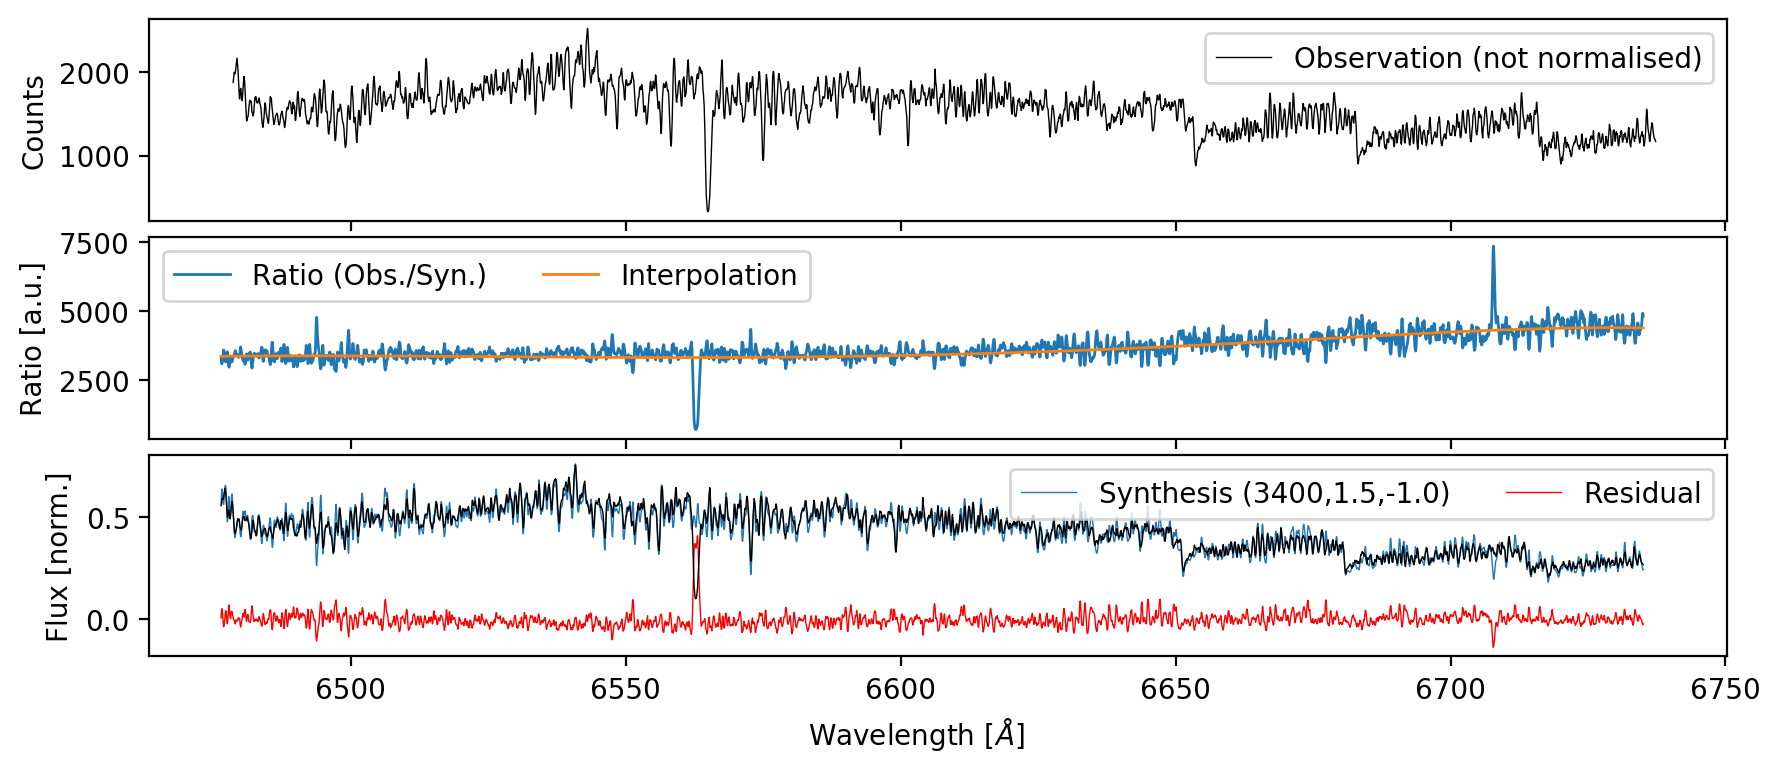
\includegraphics[width=\textwidth]{figures/Nuisance_example.png}
 \caption{
 \textbf{Example of normalisation for GALAH DR4 for a model spectrum that is selected during the label optimisation.}
 \textbf{Panel (a):} Observed spectrum (counts) of star 2MASS XYZ.
 \textbf{Panel (b):} Ratio (blue) of observed spectrum and model spectrum as well as Chebychev polynomial fit (orange).
 \textbf{Panel (c):} Normalised observed spectrum (black) compared to the model spectrum (blue). Residuals (red) can then be used as input for the likelihood function.
 }
 \label{fig:ratio_normalisation}
\end{figure}

For each CCD, the reduction has found the most suitable wavelength solution, linking pixels with actual wavelengths, based on the ThXe arc lines. In GALAH DR3 \citep{Buder2021}, we have found several issues for spectra, where not enough ThXe lines could be used to constrain the wavelength solution. Improvements have been made for the new reduction version to improve the number of useful ThXe lines. Two additional pieces of information are, however, unused by the reduction pipeline, namely (i) the telluric lines\footnote{\SB{Check with Janez if that is actually still true!}} that are present throughout GALAH spectra and (ii) the absorption lines of the stellar spectra. Both hold valuable information, as their position (in rest wavelength) is known very well.

The reduction is providing spectra and other parameters in an array of $n$ pixels, that is linked to wavelengths $\lambda_n$ through a linear function
\begin{align} \label{eq:wavelength_solution}
    \lambda (n) = \lambda_0 + n \cdot \Delta_\lambda.
\end{align}
In particular, for each CCD, the pipeline reports $\lambda_0$ as \texttt{cdelt} and $\Delta_\lambda$ as \texttt{CRVAl}.\footnote{\SB{Can we take into account uncertainties on these values through the pipeline? e.g. rms?}}
Because we can directly compare to model spectra with a perfect wavelength solution, we therefore allow these eight values (two for each of the four CCDs) to be fitted by our analysis pipeline.

\SB{Could this be degenarate with \vrad. Could be solved by (i) keeping one CCD fixed or (ii) adding a fit to the telluric lines as well, because we know their dependence on wavelength!}

\subsection{Finding the most likely set of stellar labels} \label{subsec:finding_best_labels}

To find the most set of stellar labels that best describe the data at hand, we need to either (i) maximise/sample the likelihood functions
(Eqs.~\ref{eq:likelihood_spectroscopic}, \ref{eq:likelihood_photoastrometric}, or \ref{eq:likelihood_asteroseismic}) or maximise/sample the posterior functions (Eq.~\ref{eq:posterior_s}-\ref{eq:posterior_spa}).

In addition to the parameters included in these functions, we need to optimise the nuisance parameters of \vrad as well as the wavelength solution for the four CCDs (Eq.~\ref{eq:wavelength_solution}).

\SB{MCMC from here?}

\begin{figure*}[hbt!]
 \centering
 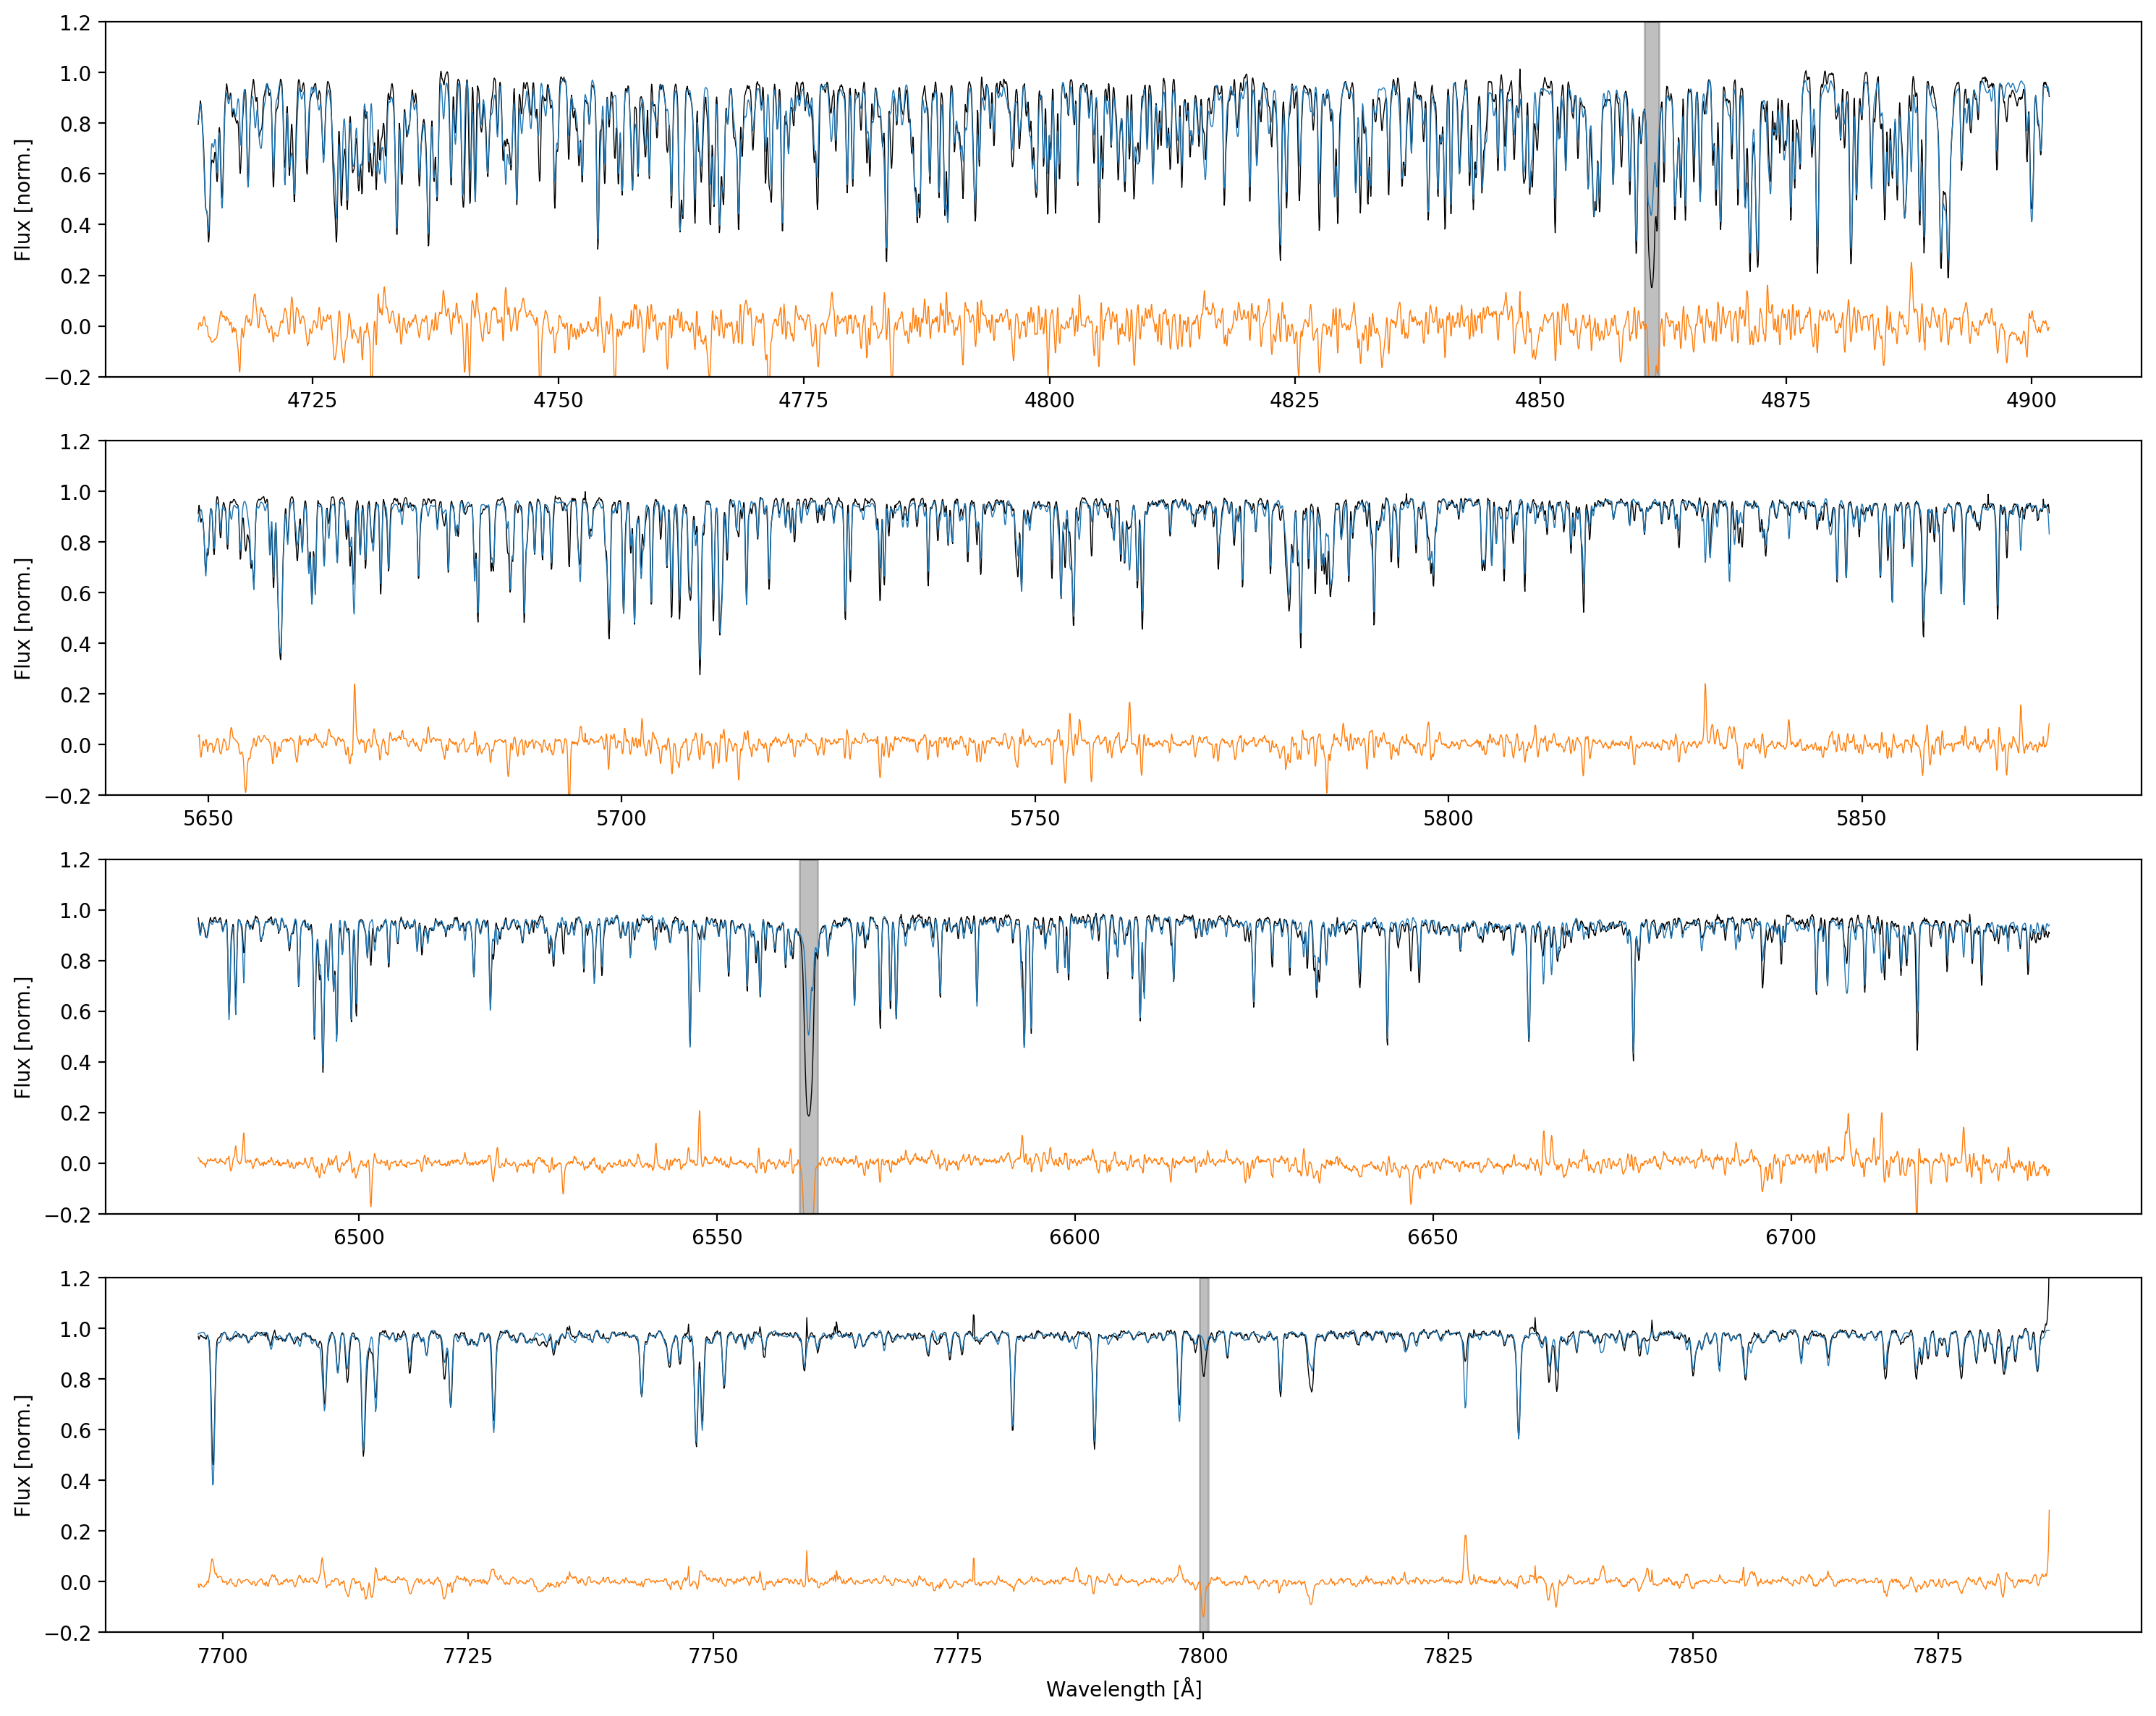
\includegraphics[width=\textwidth]{figures/150606003401143_mcmc_median.png}
 \caption{
 \textbf{Example of best-fit model spectrum (blue) for the observed spectrum (black) of 2MASS 16103957-2602249 for the 4 CCDs of HERMES.}
 Residuals are shown in orange. Grey areas show parts of the spectrum that were neglected (masked) while fitting.
 }
 \label{fig:best_fit_spectrum}
\end{figure*}

\subsubsection{Masking of spectrum pixels}

We have analysed the difference between the observed Solar spectrum by \citet{Hinkle2000} and a synthetic spectrum with Solar parameters and abundances. In detail, we created a synthetic spectrum with $T_\text{eff} = 5772\K$, $\log g = 4.438\dex$, $\mathrm{[Fe/H]} = 0.00\dex$, $v_\text{mic} = 1.06\kms$, $v \sin i = 1.6\kms$, $v_\text{mac} = 4.2\kms$ \citep{Prsa2016, Jofre2017}, and $\mathrm{[X/Fe]} = 0.00\dex$ for the default Solar abundance pattern for \marcs by \citet{Grevesse2007}. We have identified all lines that showed differences of the normalised flux of more than $0.1$, lines where either a synthetic line or an observed one was completely missing, or lines that were significantly misaligned. Examples of these masks are shown in Fig.~\ref{fig:example_masking_sun}.

\begin{figure*}[hbt!]
 \centering  
 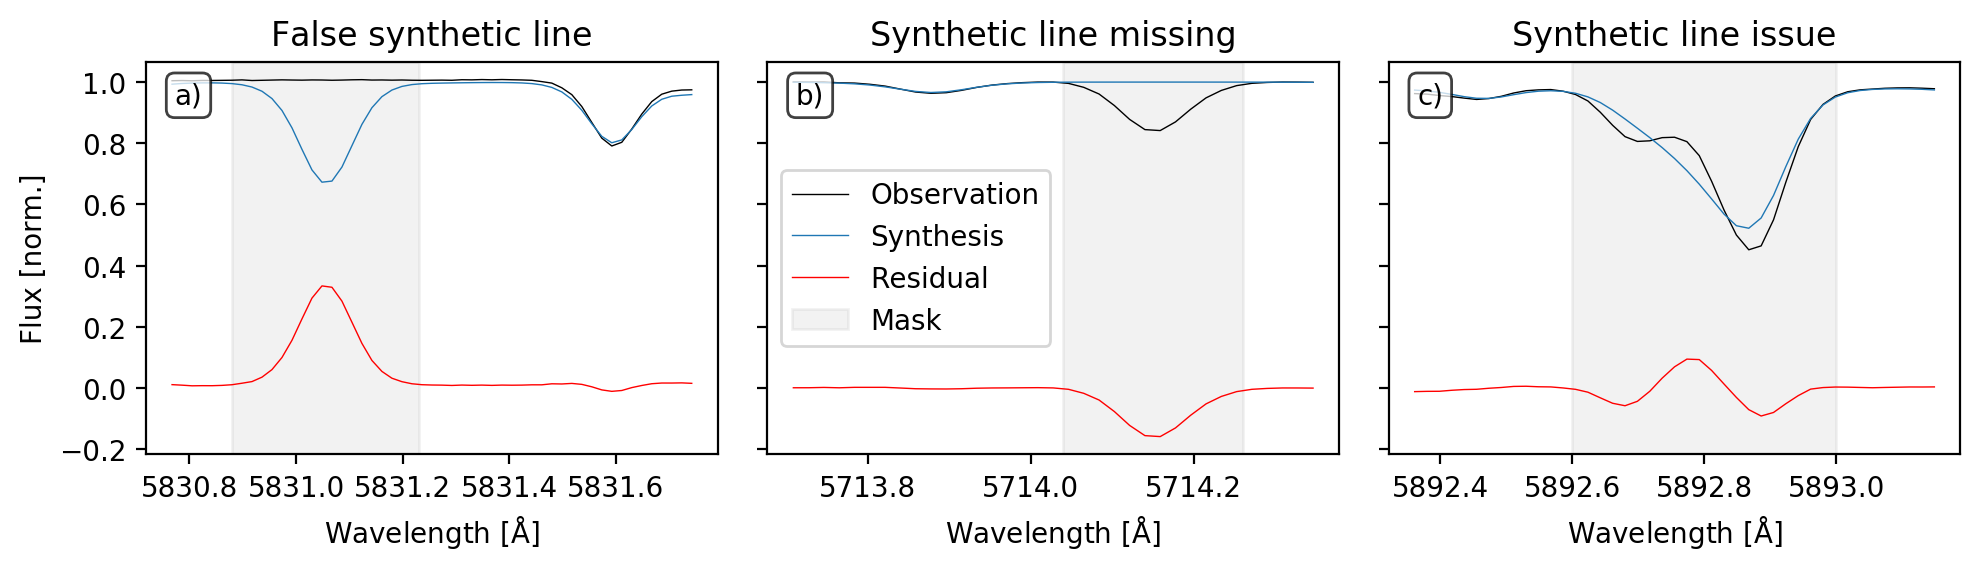
\includegraphics[width=\textwidth]{figures/example_masking_sun.png}
\caption{\textbf{Examples of masks applied to unreliable pixels for the spectrum fitting, that is the minimisation of residuals (red) between observation (black) and synthesis (blue).} \textbf{Panel a)} showing a strong synthetic line, where no line is observed in the Sun. \textbf{Panel b)} showing an observed line without any line being synthesised. \textbf{Panel c)} showing significant disagreement between the two observed lines and the synthesis.} \label{fig:example_masking_sun}
\end{figure*}

\newpage
\section{POST-PROCESSING} \label{sec:post_processing}

\subsection{Abundance detection or upper limit}

Our pipeline will find the most suitable model and in particular set of abundances for the given observation.

That does, however, not necessarily mean that the abundance of each element is actually well determined, because lines of the element may actually not be detected.

For each element, we therefore run a post-processing routine to estimate if the measured abundance is indeed significant compared to the uncertainty of the spectrum.

For each star, we therefore take the best-fit model and assess the change in the model spectrum when changing one abundance at a time.

\subsection{Flagging of problematic measurements}

\SB{Flag if parameters outside of the range of \TheCannon (e.g. \vsini$ > 30 \kms$, see Sec.~\ref{subsubsec:polynomials})}

\SB{Flag if parameters are outside of convex hull of isochrone grid, when using photoastrometric information. Also note that we have cut away \Teff above $10,000\K$ and \logg above $6\dex$.}

\newpage
\section{VALIDATION} \label{sec:validation}

\SB{Can we be sure, that we are interpolating properly between different models of \TheCannon?}

\newpage $\,$ \newpage
\section{CONCLUSIONS} \label{sec:conclusion}

%%%%%%%%%%%%%%%%%%%%%%%%%%%%%%%%%%%%%%%%%%%%%%%%%%
\section*{Acknowledgements}
%%%%%%%%%%%%%%%%%%%%%%%%%%%%%%%%%%%%%%%%%%%%%%%%%%

We acknowledge the traditional owners of the land on which the AAT and ANU stand, the Gamilaraay, the Ngunnawal and Ngambri people. We pay our respects to elders past, present, and emerging and are proud to continue their tradition of surveying the night sky in the Southern hemisphere.
This work was supported by the Australian Research Council Centre of Excellence for All Sky Astrophysics in 3 Dimensions (ASTRO 3D), through project number CE170100013.

\section*{Facilities}

\textbf{AAT with 2df-HERMES at Siding Spring Observatory:}
The GALAH Survey is based data acquired through the Australian Astronomical Observatory, under programs: A/2013B/13 (The GALAH pilot survey); A/2014A/25, A/2015A/19, A2017A/18 (The GALAH survey phase 1), A2018 A/18 (Open clusters with HERMES), A2019A/1 (Hierarchical star formation in Ori OB1), A2019A/15 (The GALAH survey phase 2), A/2015B/19, A/2016A/22, A/2016B/10, A/2017B/16, A/2018B/15 (The HERMES-TESS program), and A/2015A/3, A/2015B/1, A/2015B/19, A/2016A/22, A/2016B/12, A/2017A/14, (The HERMES K2-follow-up program). This paper includes data that has been provided by AAO Data Central (datacentral.aao.gov.au).
\textbf{\Gaia: } This work has made use of data from the European Space Agency (ESA) mission \Gaia (\url{http://www.cosmos.esa.int/gaia}), processed by the \Gaia Data Processing and Analysis Consortium (DPAC, \url{http://www.cosmos.esa.int/web/gaia/dpac/consortium}). Funding for the DPAC has been provided by national institutions, in particular the institutions participating in the \Gaia Multilateral Agreement. 
\textbf{Other facilities:} This publication makes use of data products from the Two Micron All Sky Survey \citep{Skrutskie2006} and the CDS VizieR catalogue access tool \citep{Vizier2000}.

\section*{Software}

The research for this publication was coded in \textsc{python} (version 3.7.4) and included its packages
\textsc{astropy} \citep[v. 3.2.2;][]{Robitaille2013,PriceWhelan2018},
\textsc{astroquery} \citep[v. 0.4;][]{Ginsburg2019},
\textsc{corner} \citep[v. 2.0.1;][]{corner},
\textsc{galpy} \citep[version 1.6.0;][]{Bovy2015},
\textsc{IPython} \citep[v. 7.8.0;][]{ipython},
\textsc{matplotlib} \citep[v. 3.1.3;][]{matplotlib},
\textsc{NumPy} \citep[v. 1.17.2;][]{numpy},
\textsc{scipy} \citep[version 1.3.1;][]{scipy},
\textsc{sklearn} \citep[v. 0.21.3;][]{scikit-learn},
\textsc{statsmodels} (v. 0.10.1),
\textsc{xdgmm} (v. 1.1).
We further made use of \textsc{topcat} \citep[version 4.7;][]{Taylor2005};


% \begin{table*}
% \begin{threeparttable}
% \caption{Identified backscatter from objects in orbit and their properties}\label{satdet}
% \begin{tabular}{ c c c c c c } \toprule
% Satellite\tnote{a}   &NORAD           &Start      &End               &Mean intensity         &RCS\tnote{b}            \\
% name        &ID \#           &time (UT)       &time (UT)             & (Jy/beam)      &($m^{2}$)        \\ \midrule
% BGUSAT      & 41999 &2020-01-31 14:40:09.9  &2020-01-31 14:43:11.9  &1060  &$<$0.1       \\ 
% ISS (ZARYA) & 25544 &2020-01-31 17:17:41.9  &2020-01-31 17:19:00.9  &440  & $>$1.0      \\ 
% MAX VALIER SAT& 42778 &2020-02-03 01:18:16.9  &2020-02-03 01:20:09.9  &650  &0.1 $-$ 1.0       \\
% ISS (ZARYA) &22554 &2020-02-03 01:31:07.9  &2020-02-03 01:33:14.9  &930  &$>$1.0         \\ 
% FLOCK 3P 71 & 42024 &2020-02-01 14:16:22.9& 2020-02-01 14:18:05.9  &330  &$<$0.1       \\ 
% ISS (ZARYA) & 25544 &2020-02-02 02:18:17.9  &2020-02-02 02:20:16.9  &740  &$>$1.0 \\  
% BGUSAT      & 41999 &2020-02-02 02:18:17.9  &2020-02-02 02:20:16.9  &1010  &$<$0.1 \\ \bottomrule
% \end{tabular}
% \begin{tablenotes}
% \item[a] TLE information for predicted trajectories from space-track.org for the epoch of observation: 2020-02-01
% \item[b] Radar Cross Section (RCS) is categorised by space-track.org as: small ($<$0.1); medium (0.1 $<$ RCS $<$ 1.0); and large ($>$1.0)
% \end{tablenotes}
% \end{threeparttable}
% \end{table*}


\bibliography{bib}

\appendix

\section{Gradient Spectra}

\newpage

\subsection{Gradient Spectra for Sun-like stars}

We show the \sme gradient spectra for Sun-like stars in Figs.~\ref{fig:gradient_spectra_1931_1}--\ref{fig:gradient_spectra_1931_4}. These were created by a comparing rotationally broadened ($v \sin i = 24\kms$) median spectrum of the 3D bin with synthetic spectra, for which we increased (black) and decreased (blue) one particular label at a time. These were used to create masks in order to restrict \TheCannon to only those pixels, where the most extreme changes within our parameter limits caused less than \SB{0.001} change in normalised flux (orange dots).

\begin{figure*}[h!]
 \centering
 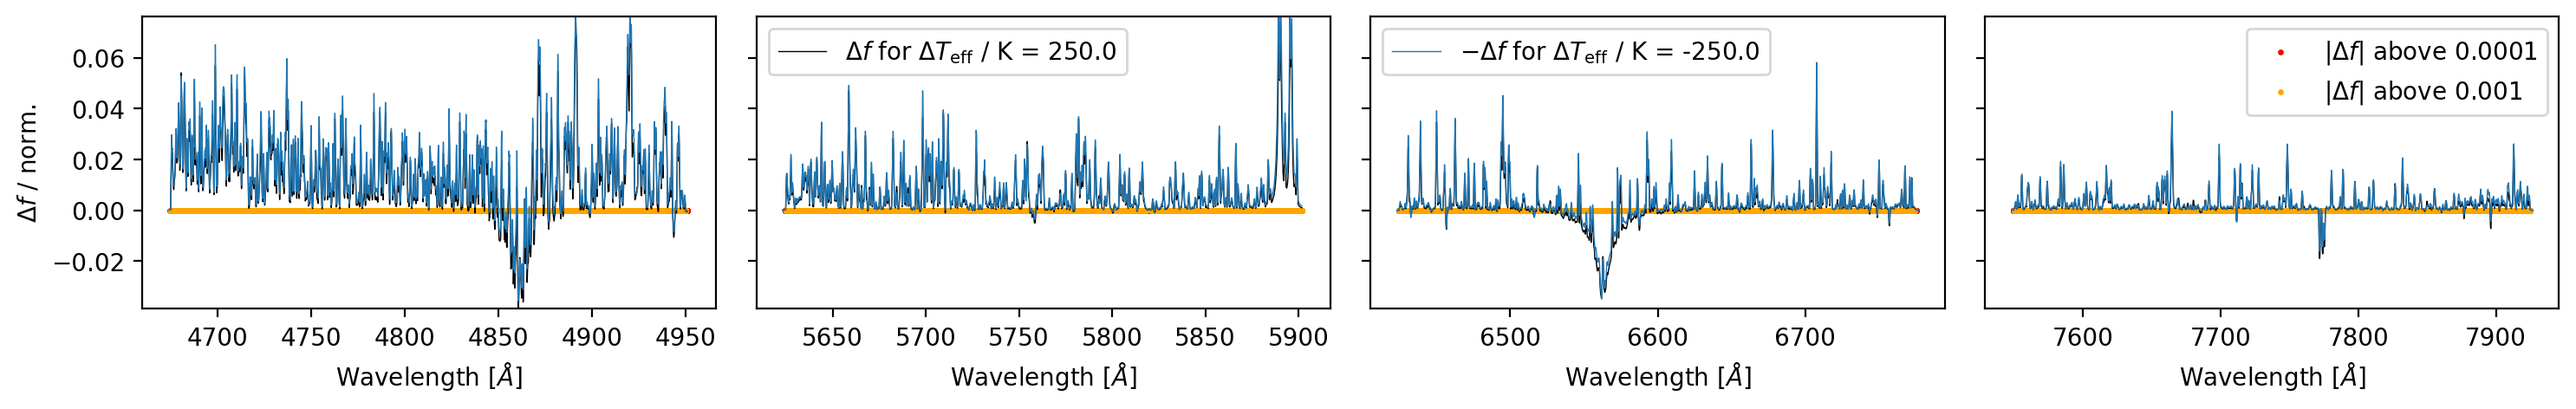
\includegraphics[width=\textwidth]{figures/gradient_spectrum_1931_teff.png}
 
\includegraphics[width=\textwidth]{figures/gradient_spectrum_1931_logg.png}
 
\includegraphics[width=\textwidth]{figures/gradient_spectrum_1931_fe_h.png}
  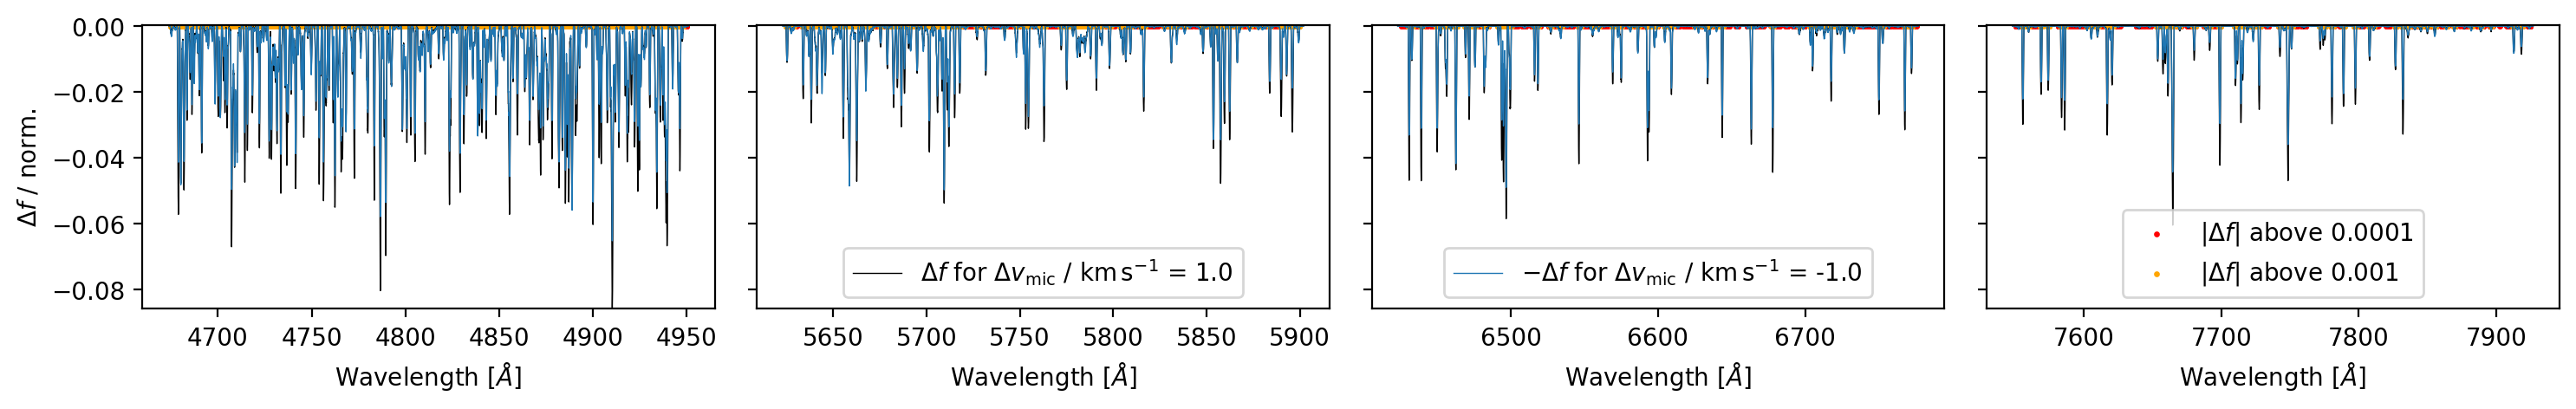
\includegraphics[width=\textwidth]{figures/gradient_spectrum_1931_vmic.png}
 
\includegraphics[width=\textwidth]{figures/gradient_spectrum_1931_li_fe.png}
 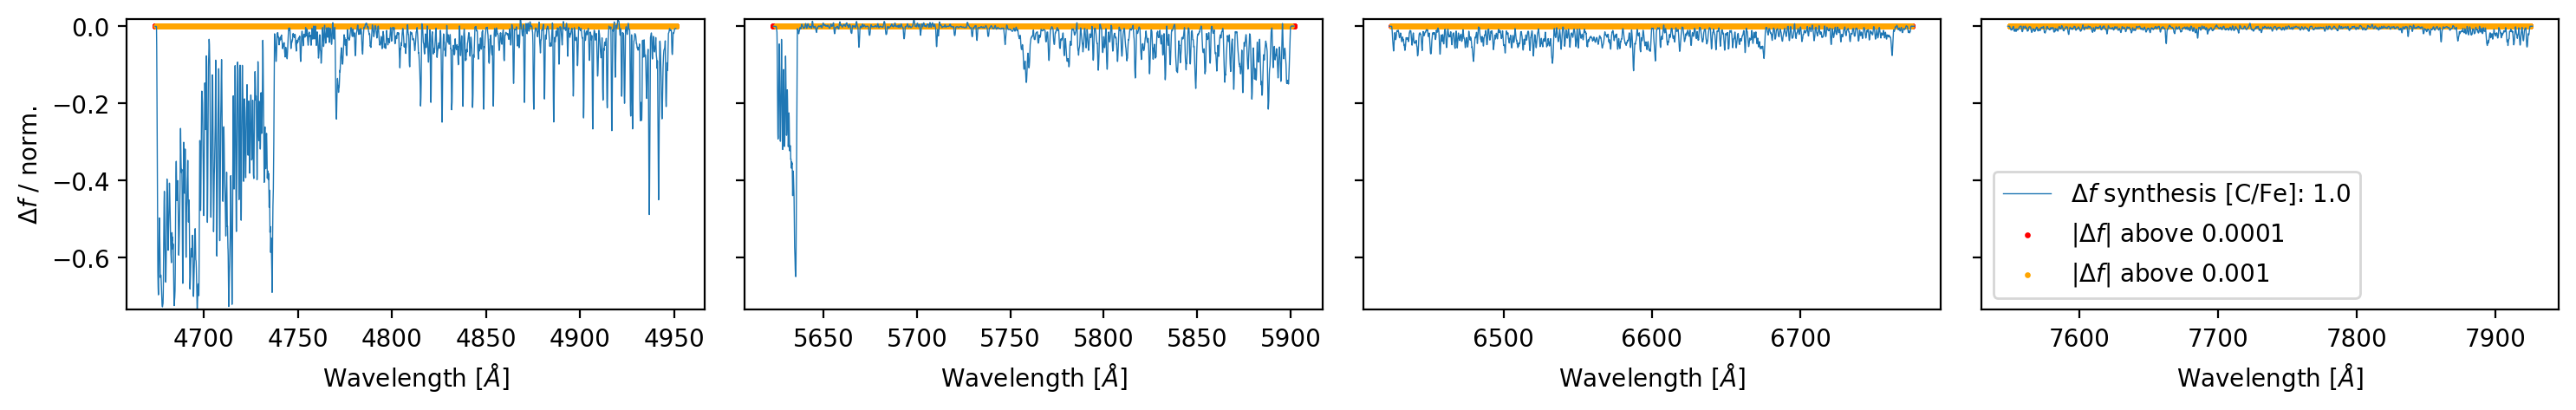
\includegraphics[width=\textwidth]{figures/gradient_spectrum_1931_c_fe.png}
 
\includegraphics[width=\textwidth]{figures/gradient_spectrum_1931_n_fe.png}

 \caption{\textbf{\sme gradient spectra for 3D bin 1931 (\Teff 5750, \logg 4.5, \feh 0.0).} Shown are differences of the normalised flux (blue) between the median synthetic spectrum and synthetic spectra increased by a certain value for each stellar label (see legend for details). Red dots indicate pixels where the absolute change of flux was above 0.0001, orange ones those pixels with changes above 0.001.
} \label{fig:gradient_spectra_1931_1}
\end{figure*}

\begin{figure*}[hbt!]
 \centering  
 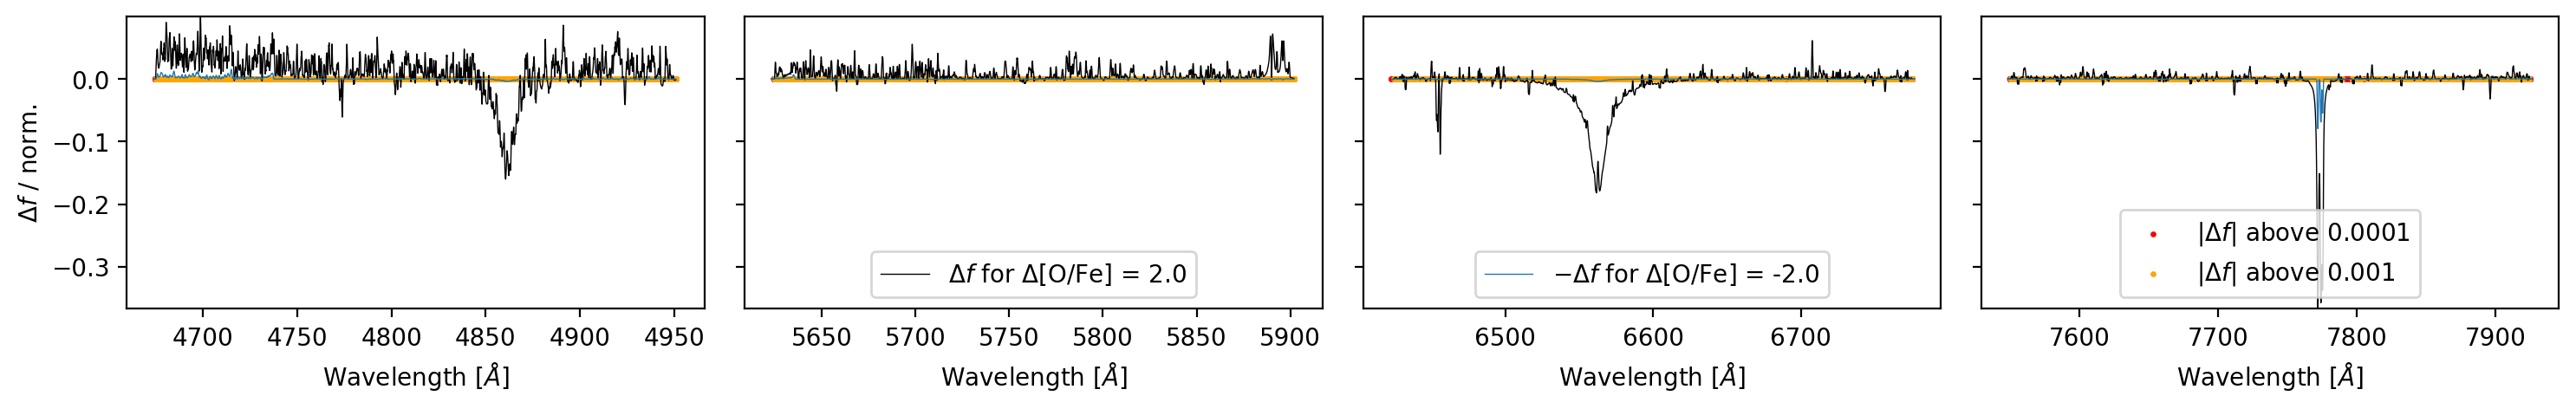
\includegraphics[width=\textwidth]{figures/gradient_spectrum_1931_o_fe.png}
 
\includegraphics[width=\textwidth]{figures/gradient_spectrum_1931_na_fe.png}
 
\includegraphics[width=\textwidth]{figures/gradient_spectrum_1931_mg_fe.png}
 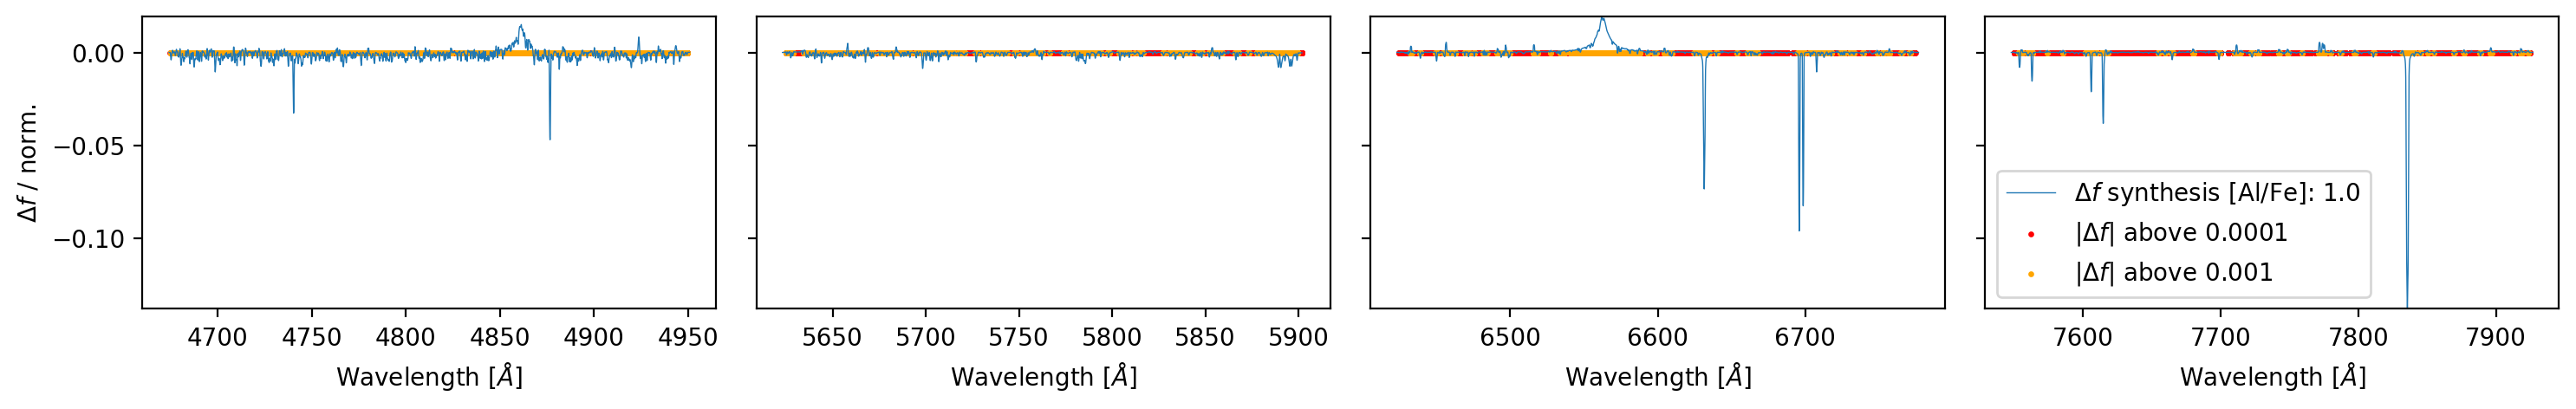
\includegraphics[width=\textwidth]{figures/gradient_spectrum_1931_al_fe.png}
 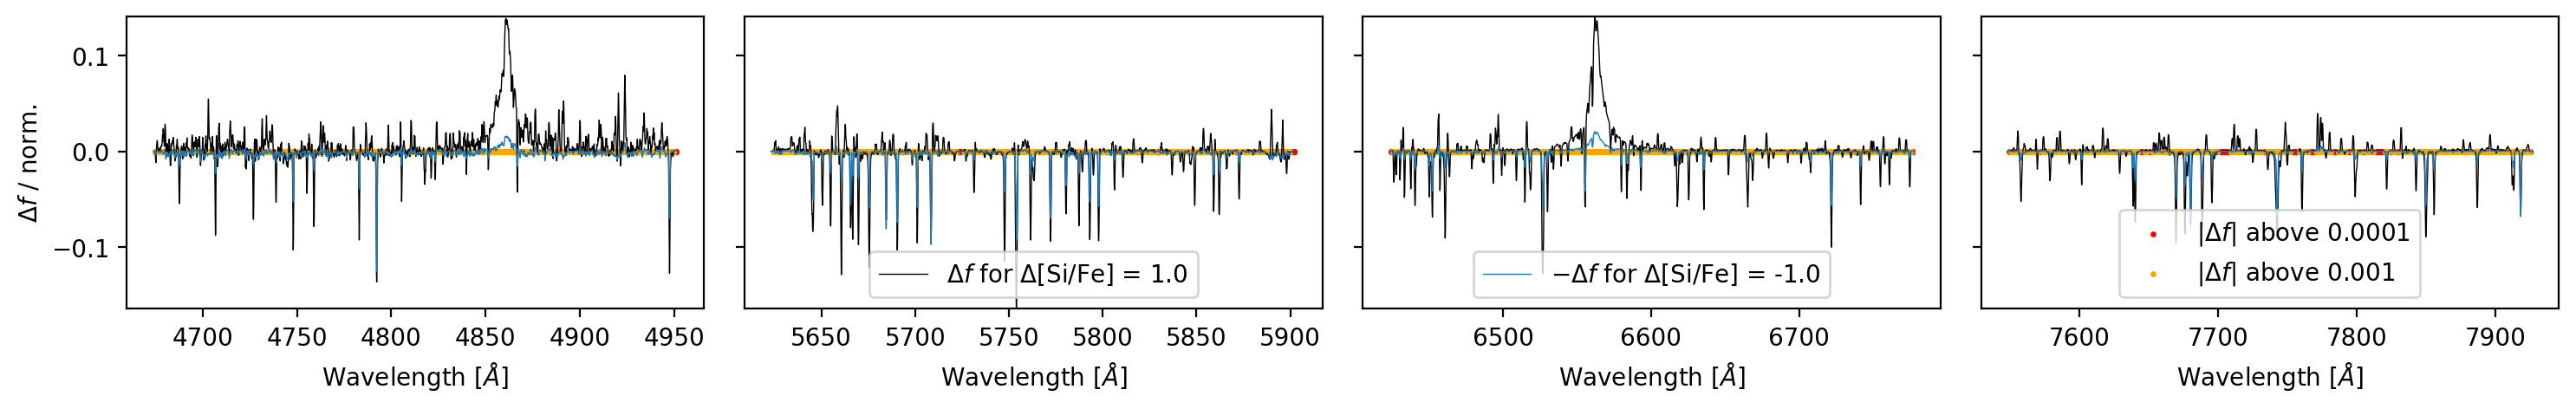
\includegraphics[width=\textwidth]{figures/gradient_spectrum_1931_si_fe.png}
 
\includegraphics[width=\textwidth]{figures/gradient_spectrum_1931_k_fe.png}
 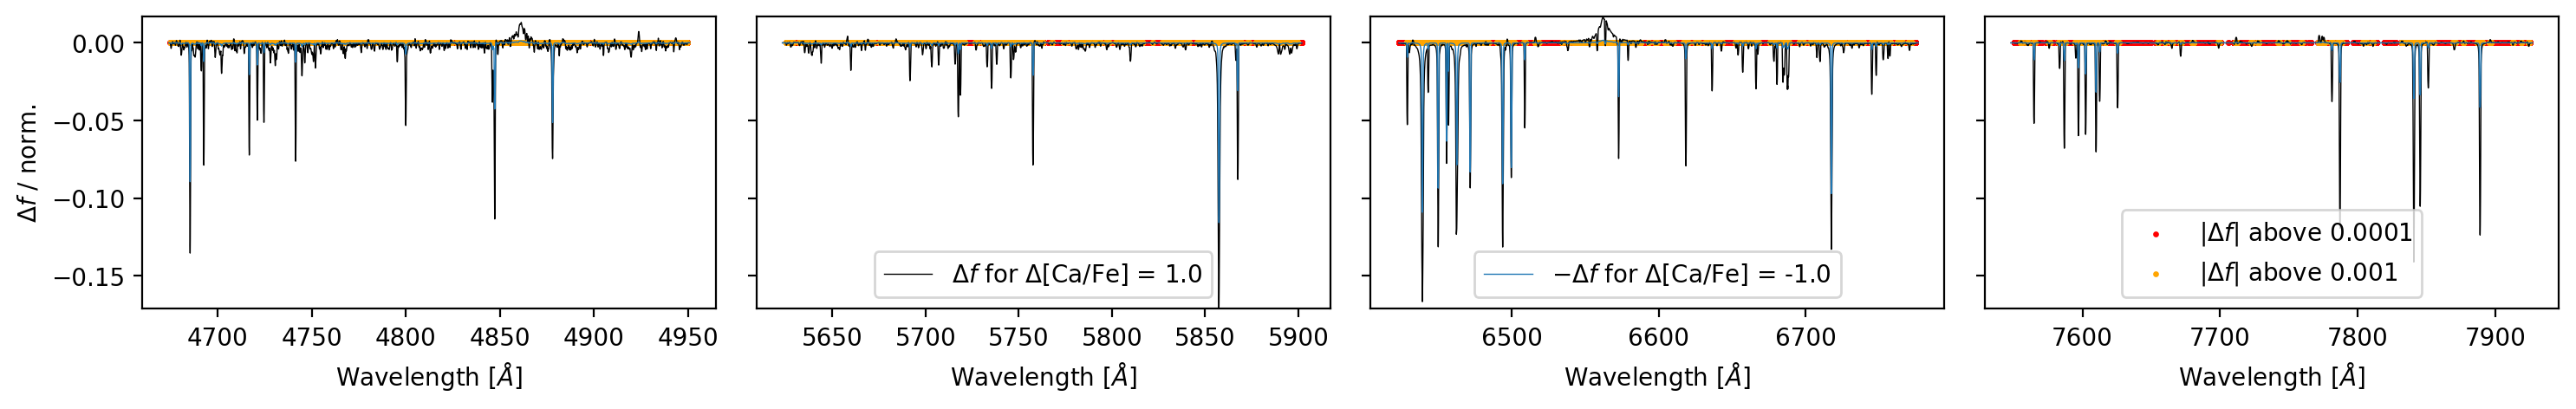
\includegraphics[width=\textwidth]{figures/gradient_spectrum_1931_ca_fe.png}
 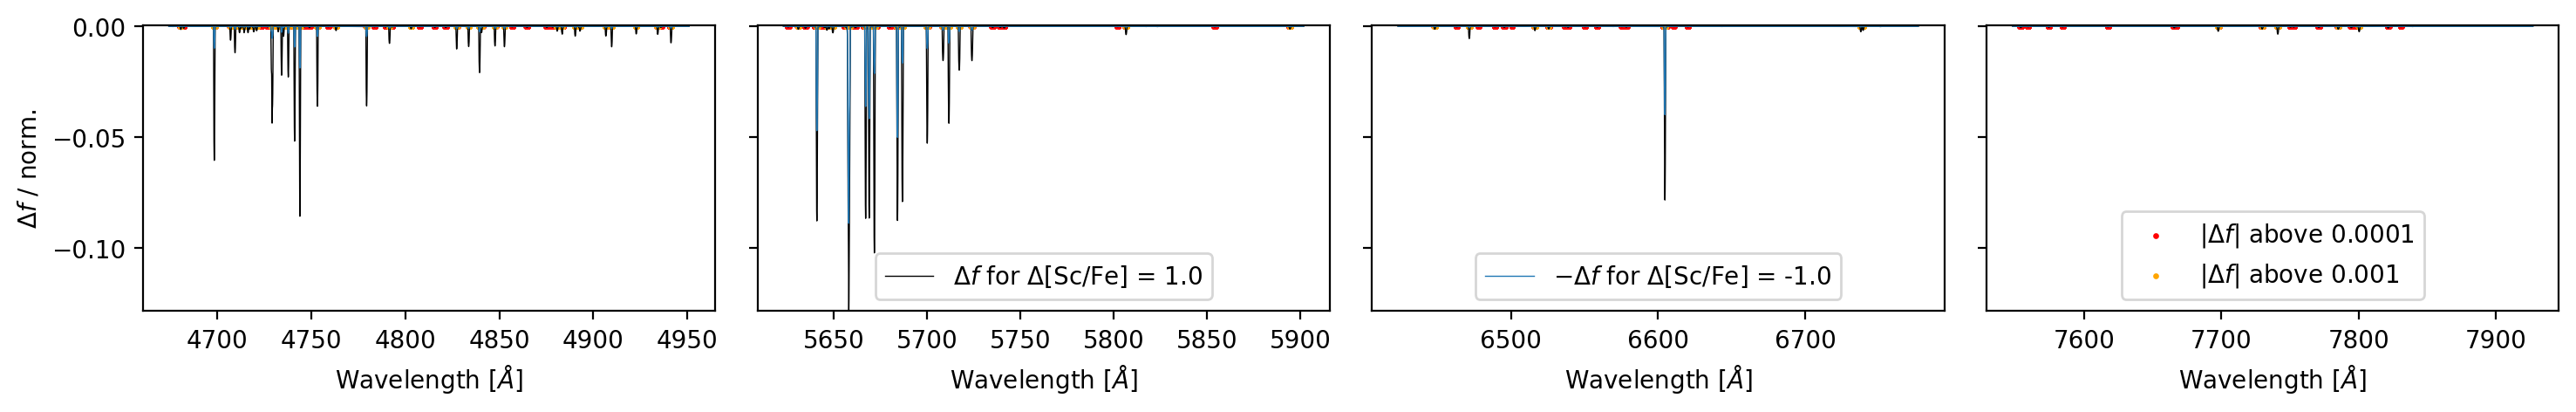
\includegraphics[width=\textwidth]{figures/gradient_spectrum_1931_sc_fe.png}
 \caption{\textbf{Continuation of Fig.~\ref{fig:gradient_spectra_1931_1}.}} \label{fig:gradient_spectra_1931_2}
\end{figure*}

\begin{figure*}[hbt!]
 \centering  
 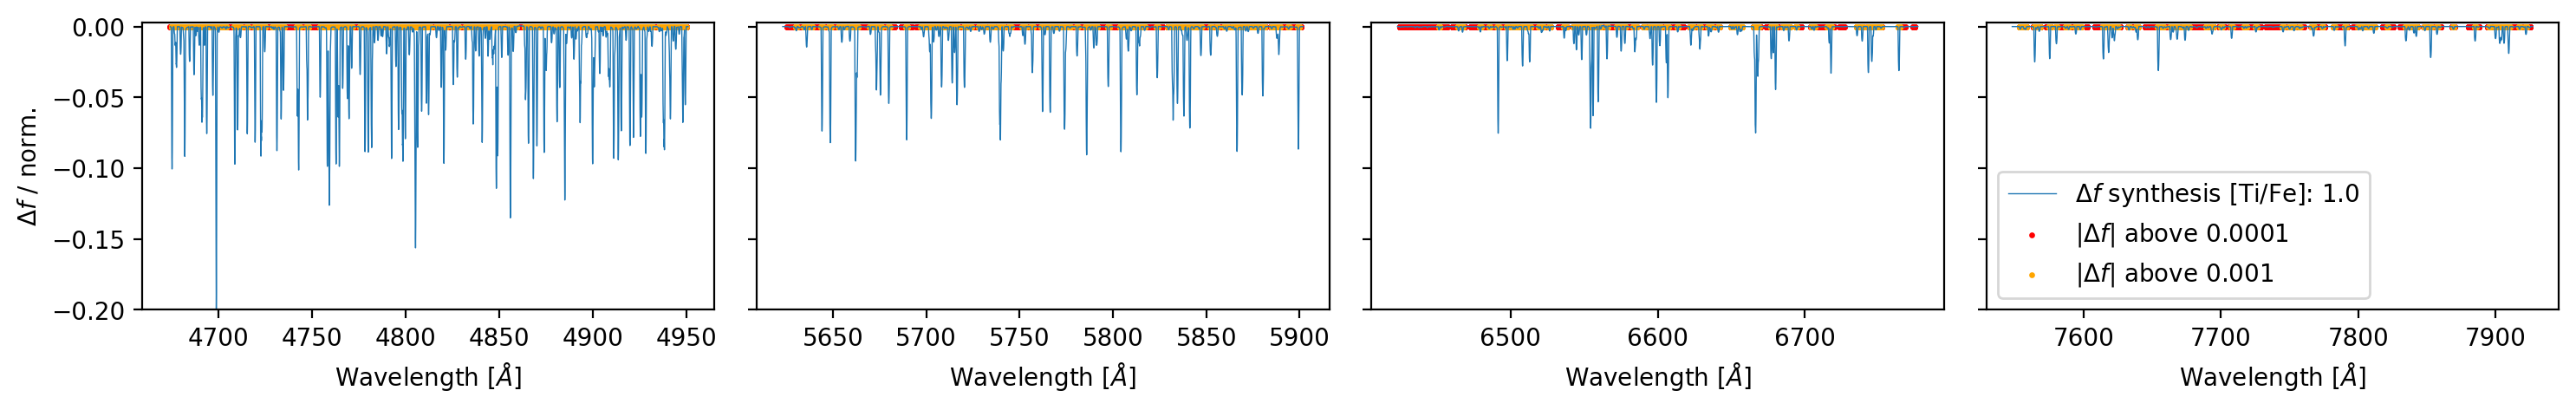
\includegraphics[width=\textwidth]{figures/gradient_spectrum_1931_ti_fe.png}
 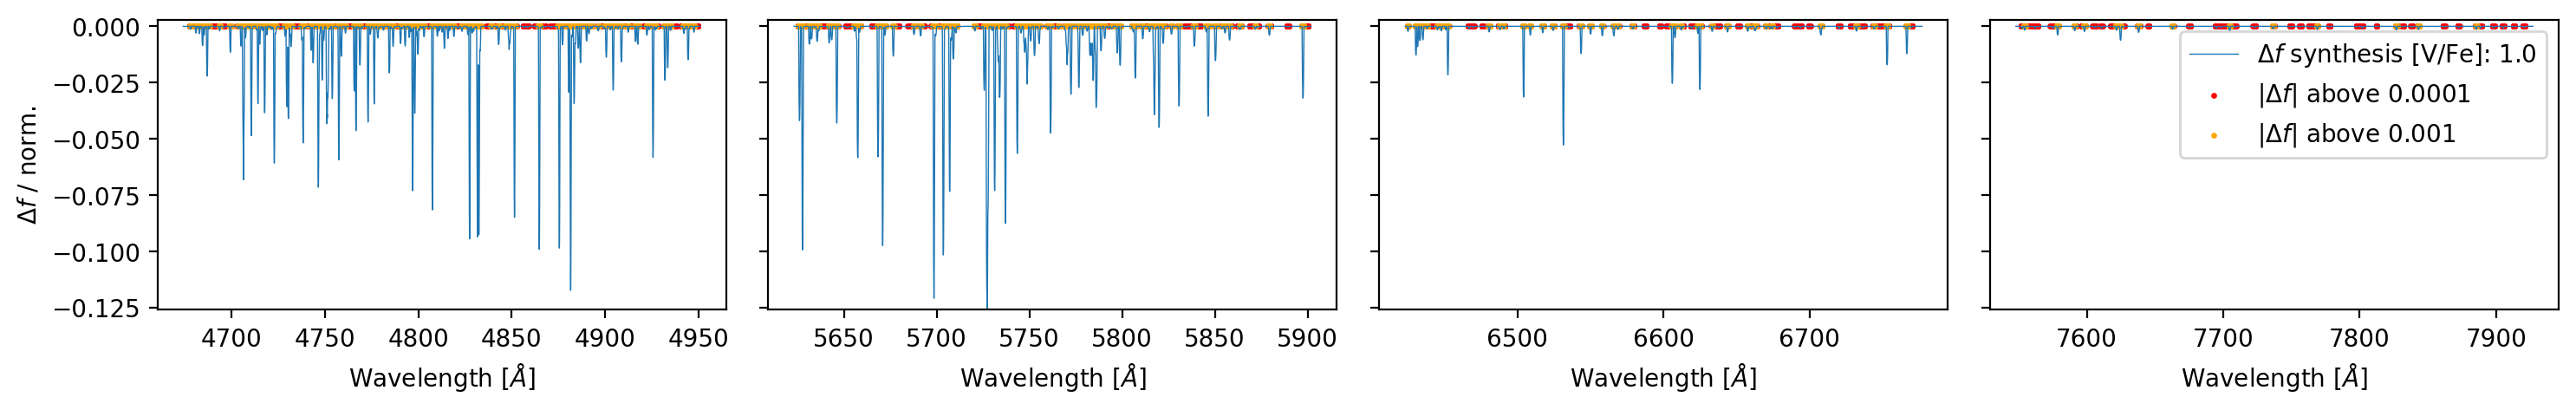
\includegraphics[width=\textwidth]{figures/gradient_spectrum_1931_v_fe.png}
 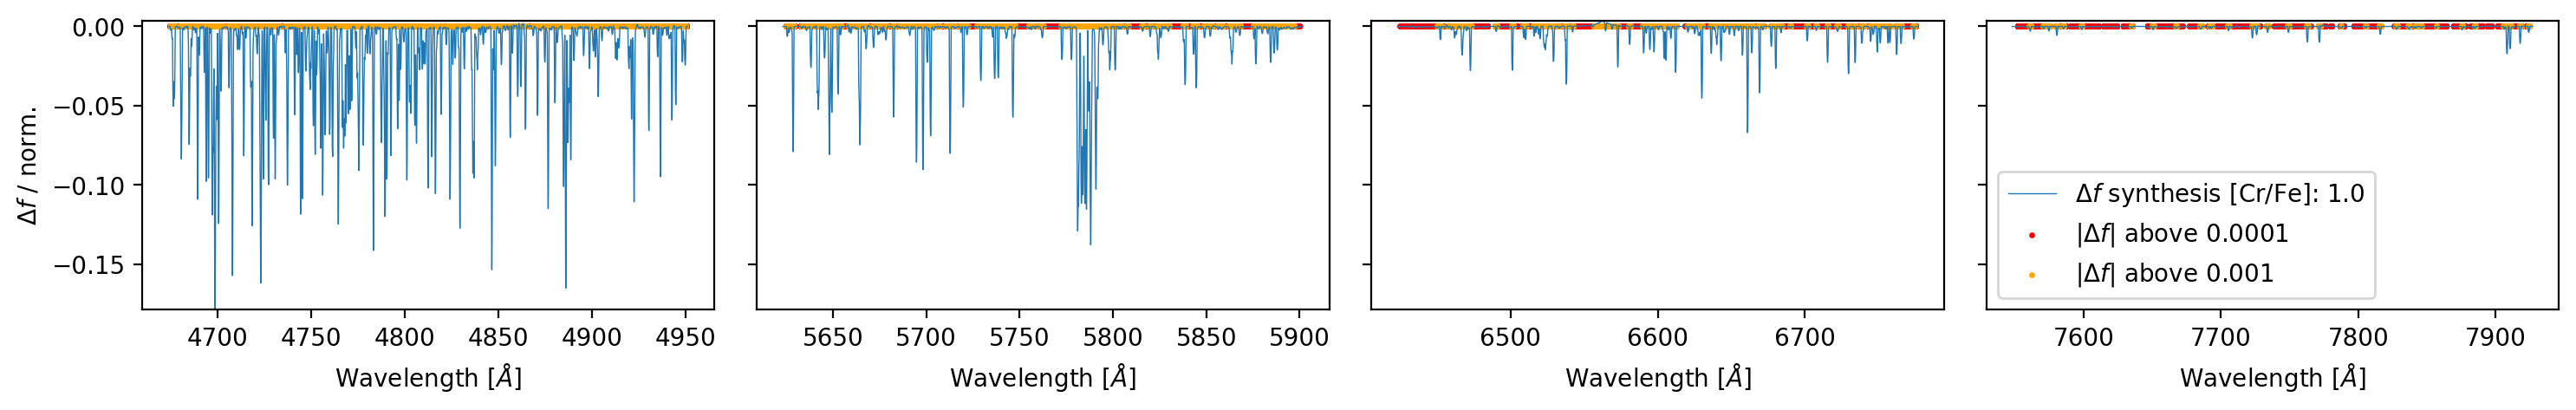
\includegraphics[width=\textwidth]{figures/gradient_spectrum_1931_cr_fe.png}
 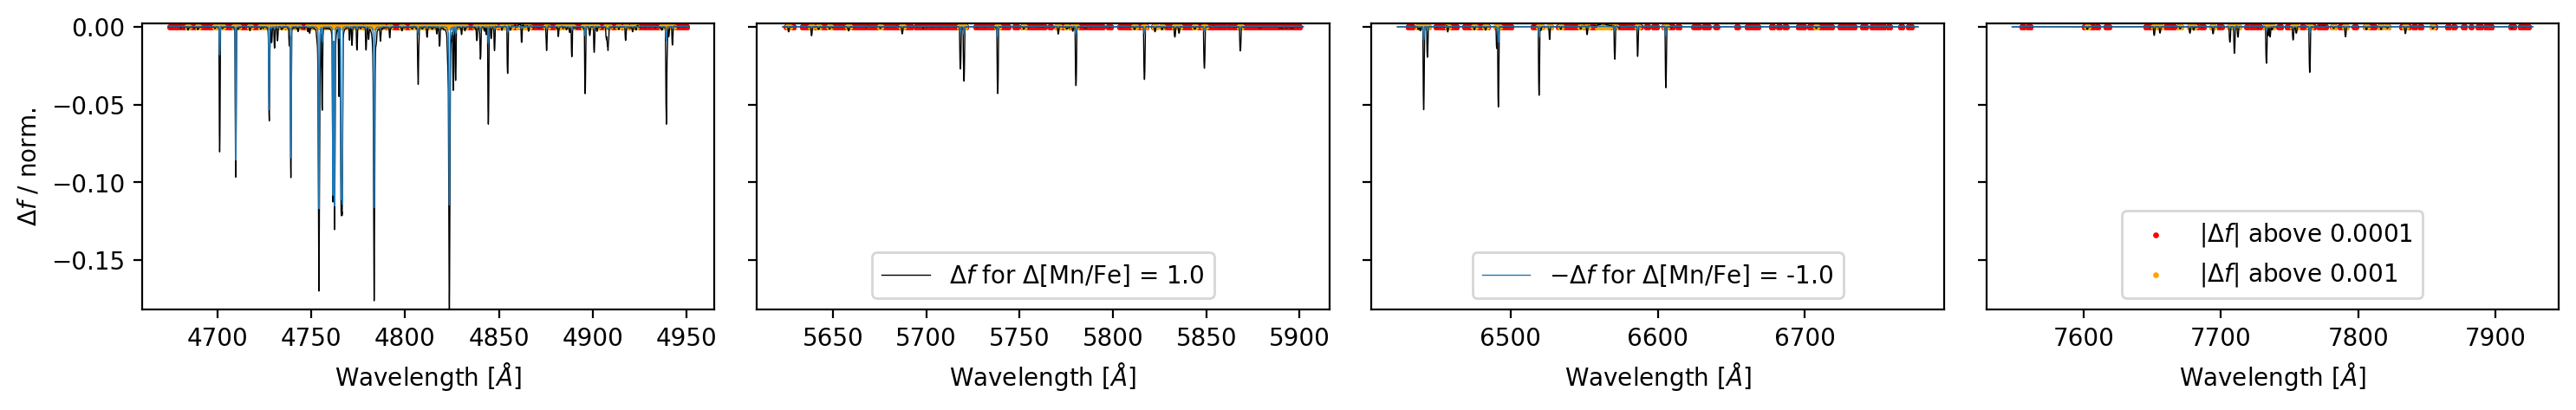
\includegraphics[width=\textwidth]{figures/gradient_spectrum_1931_mn_fe.png}
 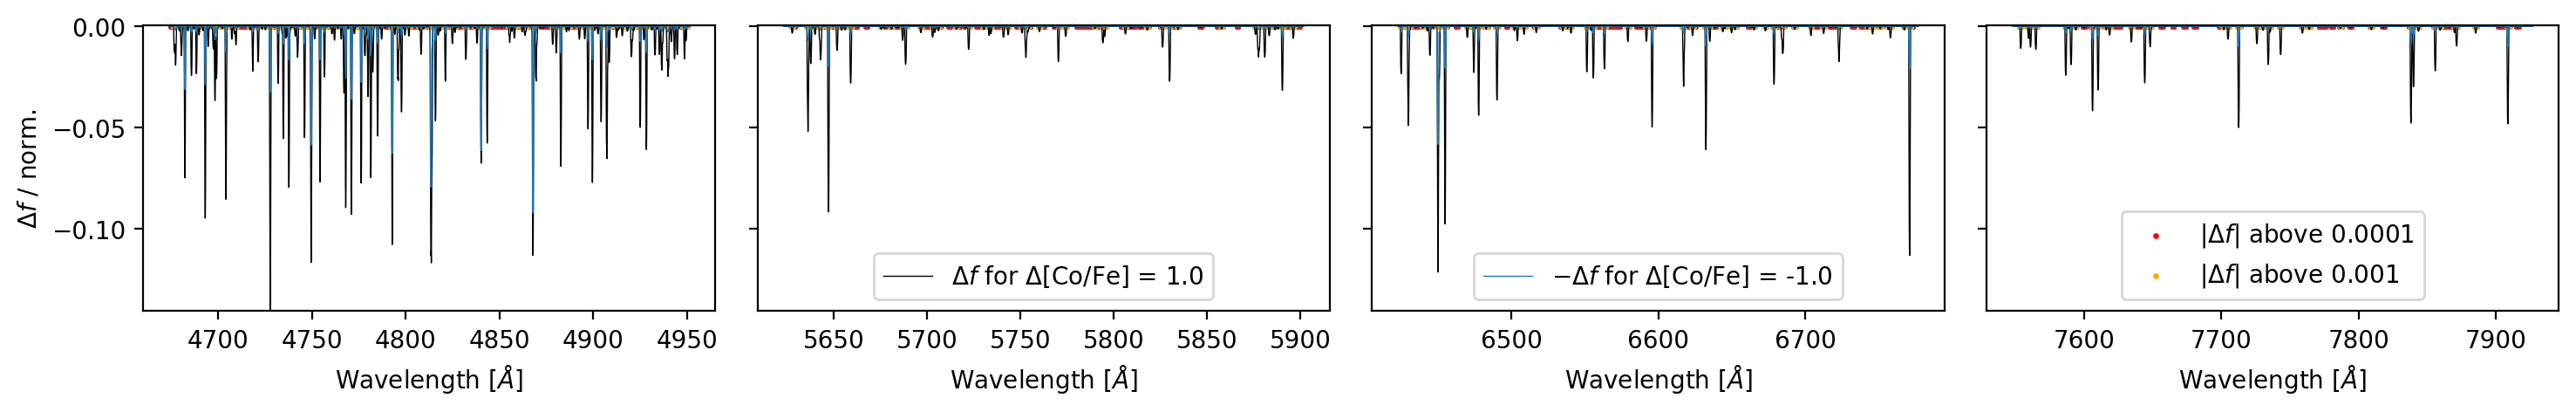
\includegraphics[width=\textwidth]{figures/gradient_spectrum_1931_co_fe.png}
 
\includegraphics[width=\textwidth]{figures/gradient_spectrum_1931_ni_fe.png}
 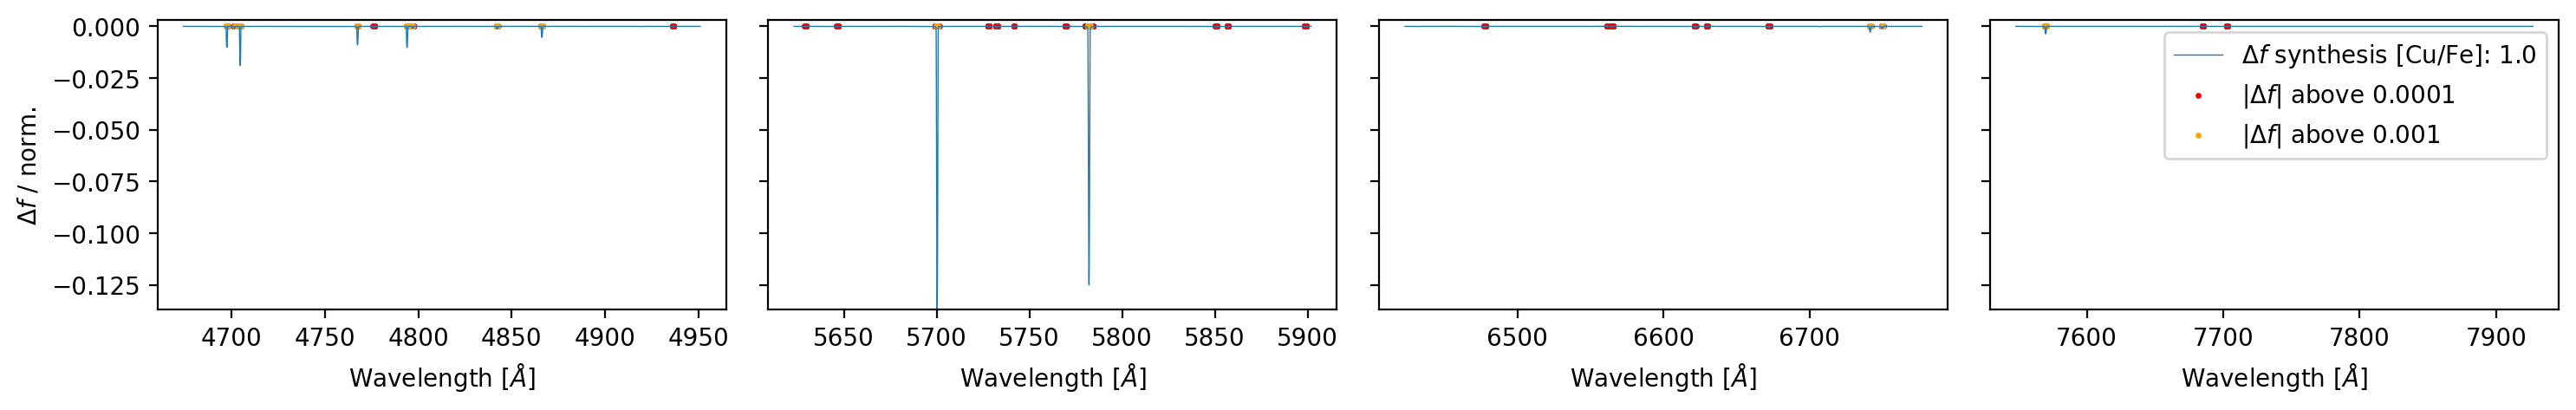
\includegraphics[width=\textwidth]{figures/gradient_spectrum_1931_cu_fe.png}
 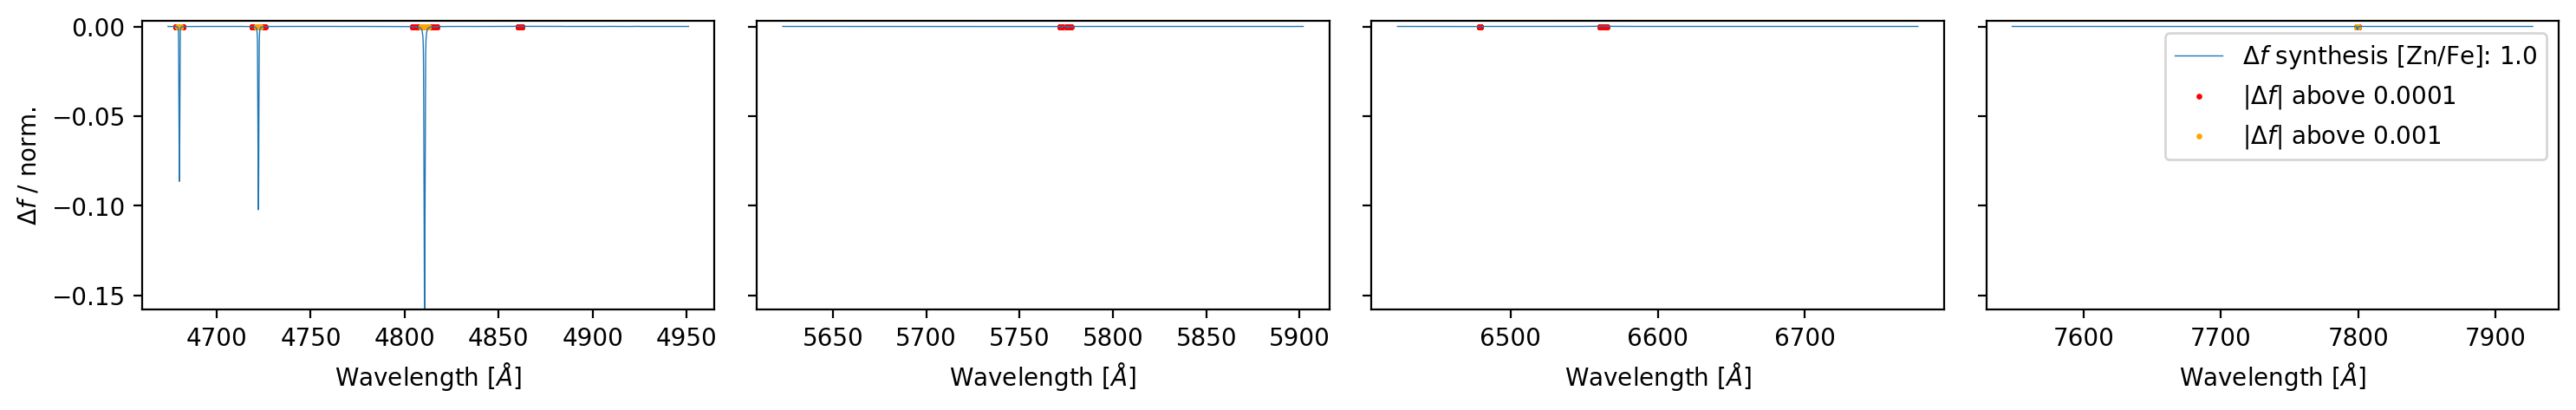
\includegraphics[width=\textwidth]{figures/gradient_spectrum_1931_zn_fe.png}
 \caption{\textbf{Continuation of Figs.~\ref{fig:gradient_spectra_1931_1} and \ref{fig:gradient_spectra_1931_2}.}} \label{fig:gradient_spectra_1931_3}
\end{figure*}


\begin{figure*}[hbt!]
 \centering  
 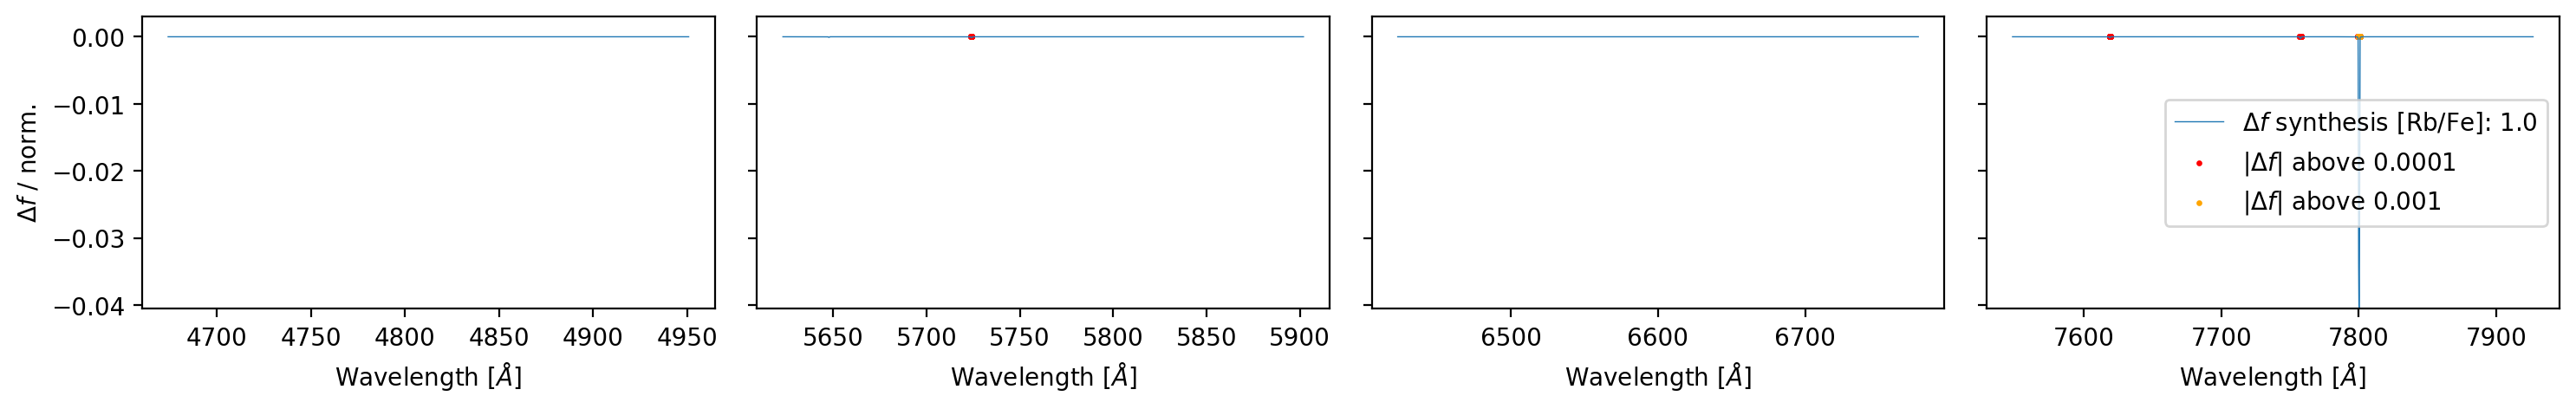
\includegraphics[width=\textwidth]{figures/gradient_spectrum_1931_rb_fe.png}
 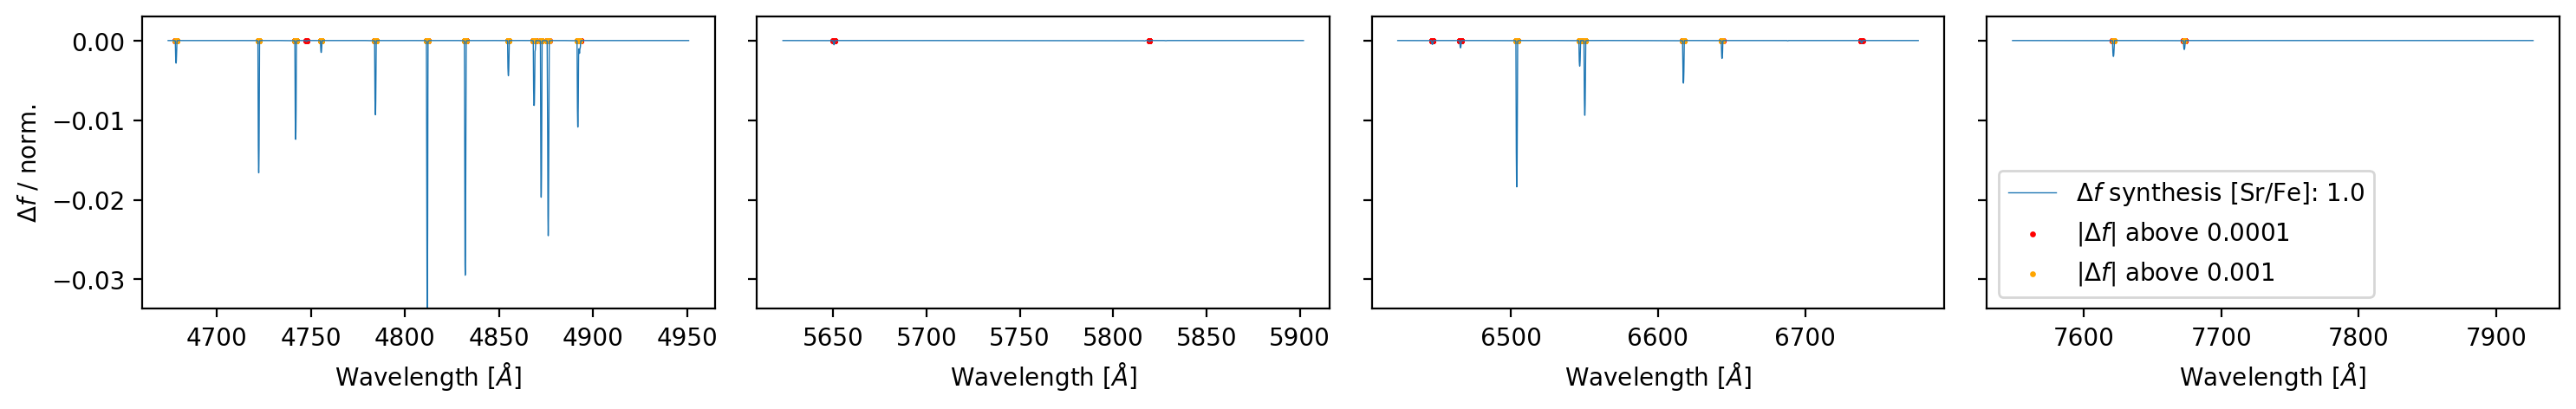
\includegraphics[width=\textwidth]{figures/gradient_spectrum_1931_sr_fe.png}
 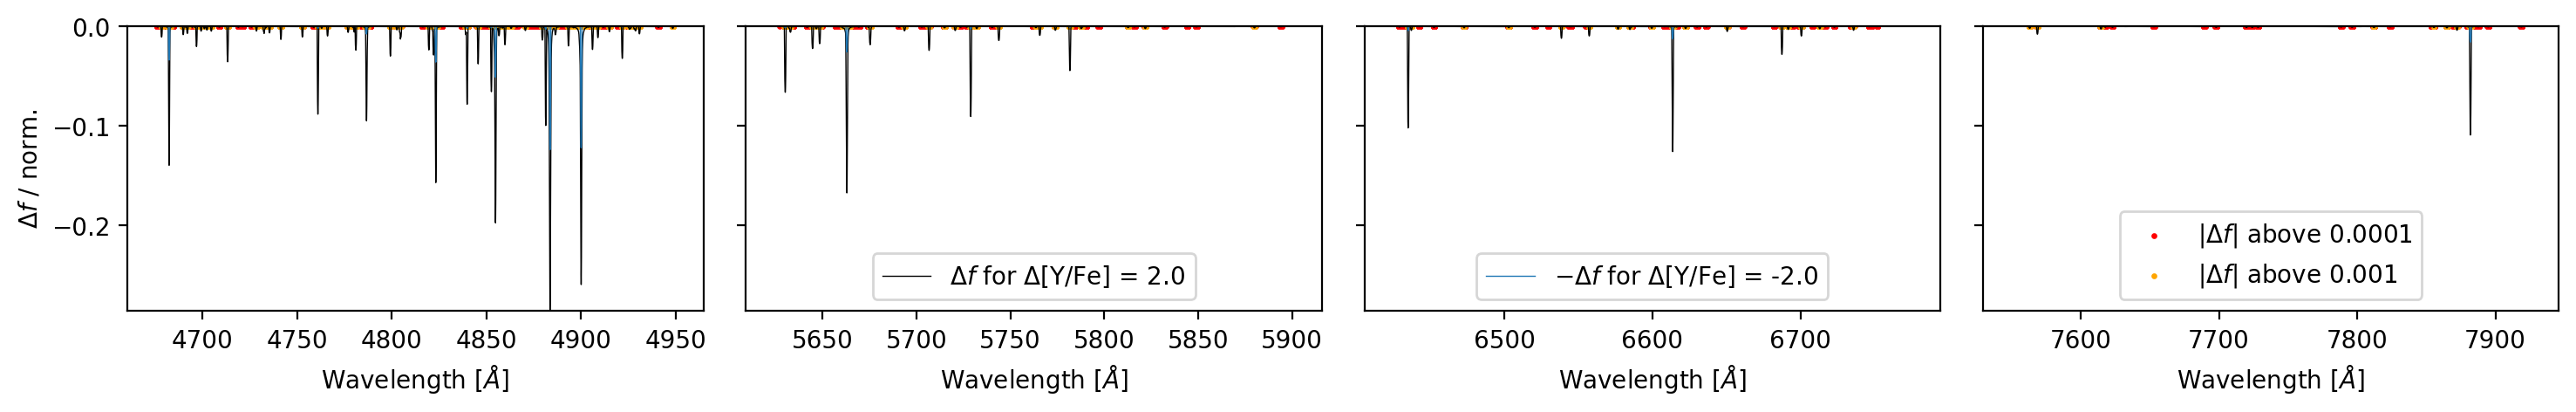
\includegraphics[width=\textwidth]{figures/gradient_spectrum_1931_y_fe.png}
 
\includegraphics[width=\textwidth]{figures/gradient_spectrum_1931_zr_fe.png}
 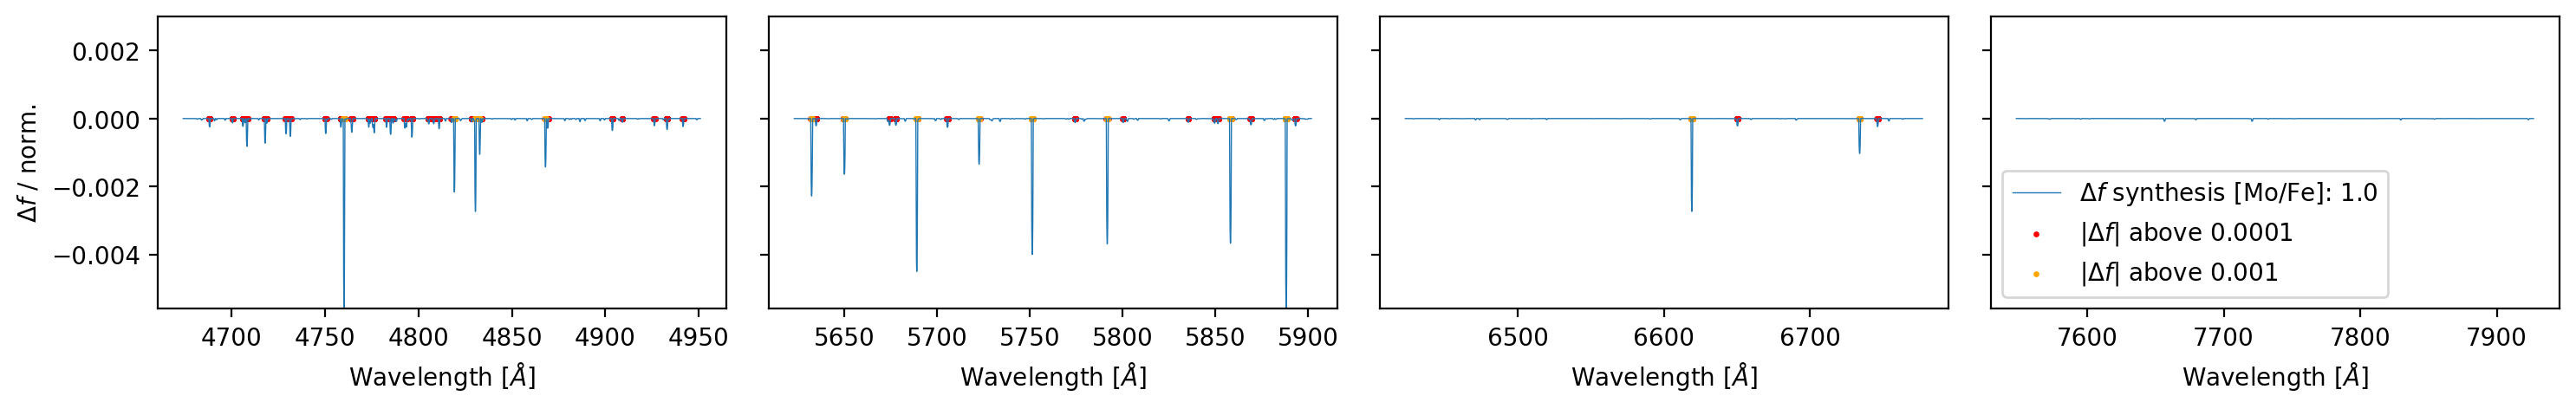
\includegraphics[width=\textwidth]{figures/gradient_spectrum_1931_mo_fe.png}
 
\includegraphics[width=\textwidth]{figures/gradient_spectrum_1931_ru_fe.png}
 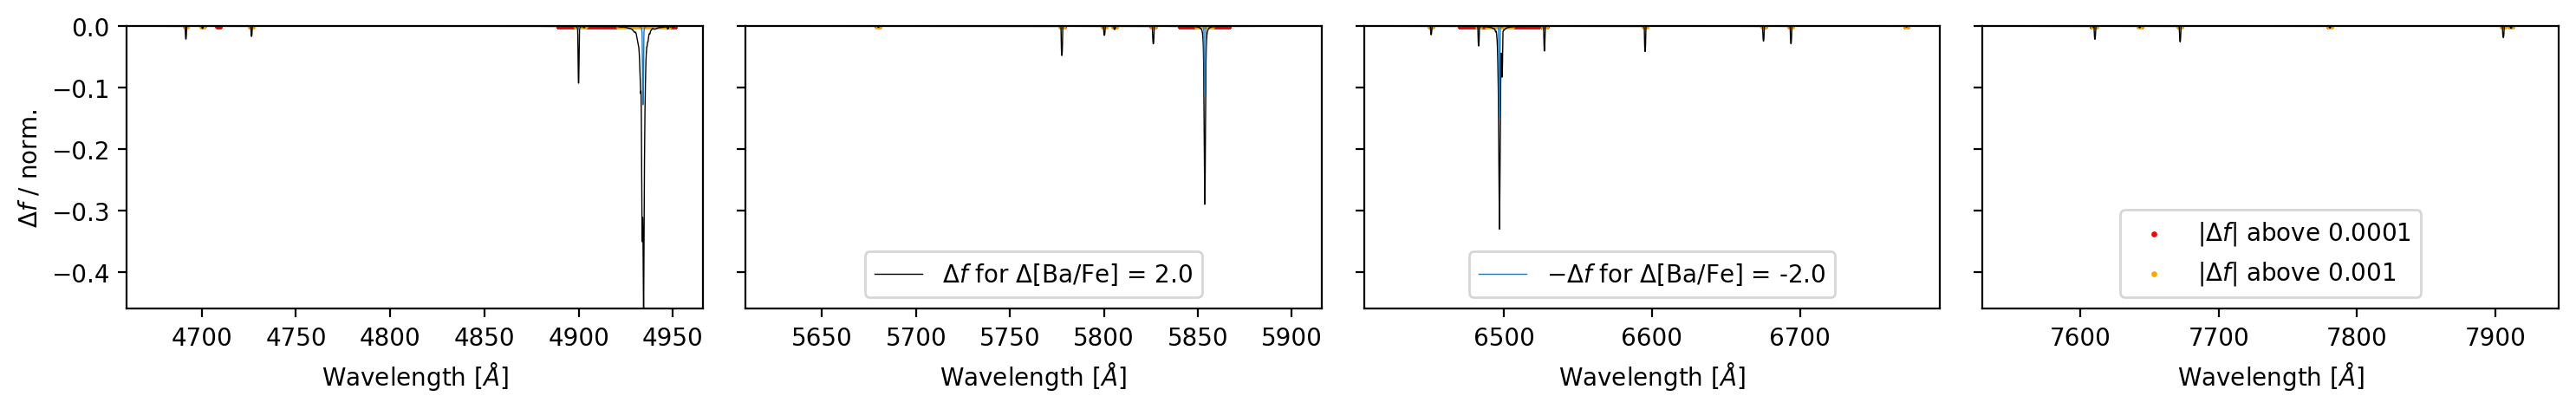
\includegraphics[width=\textwidth]{figures/gradient_spectrum_1931_ba_fe.png}
 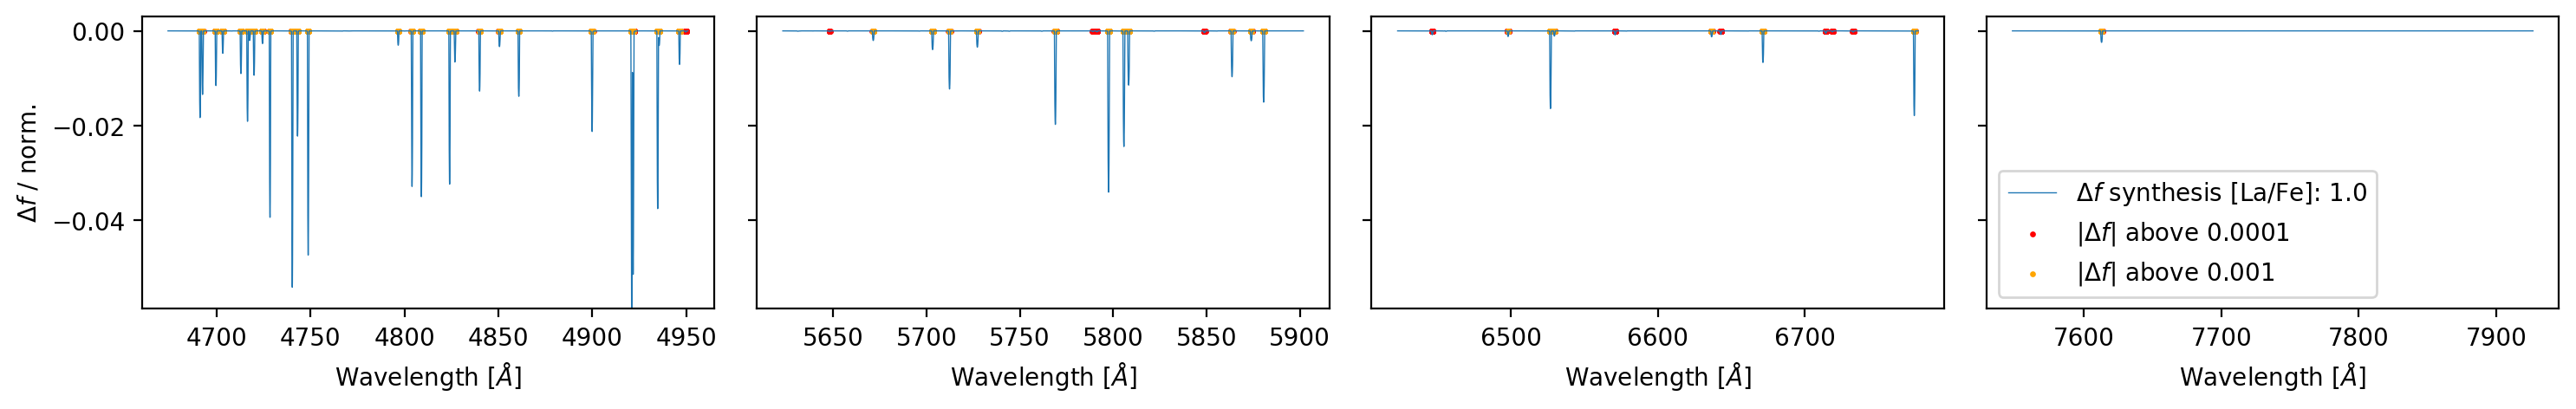
\includegraphics[width=\textwidth]{figures/gradient_spectrum_1931_la_fe.png}
 \caption{\textbf{Continuation of Figs.~\ref{fig:gradient_spectra_1931_1}--\ref{fig:gradient_spectra_1931_3}.}} \label{fig:gradient_spectra_1931_4}
\end{figure*}

\begin{figure*}[hbt!]
 \centering  
 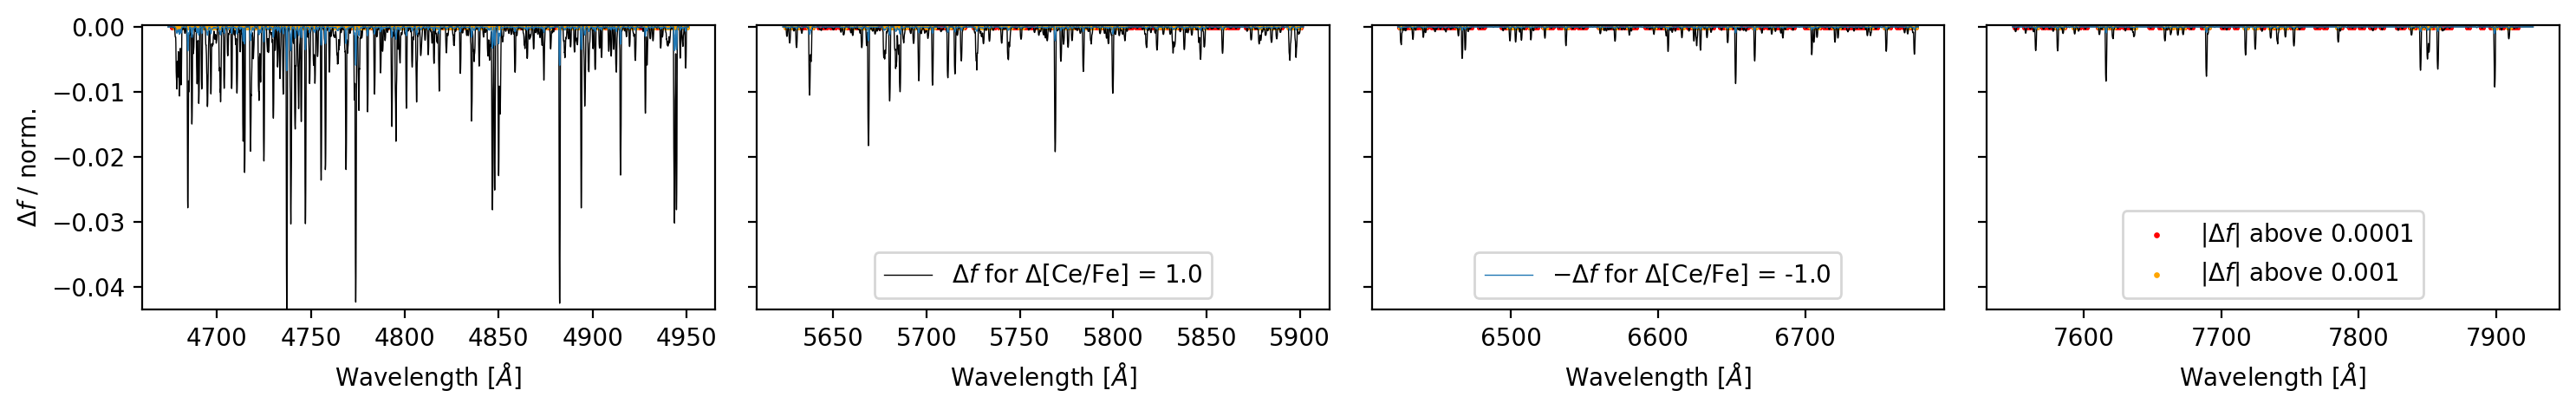
\includegraphics[width=\textwidth]{figures/gradient_spectrum_1931_ce_fe.png}
 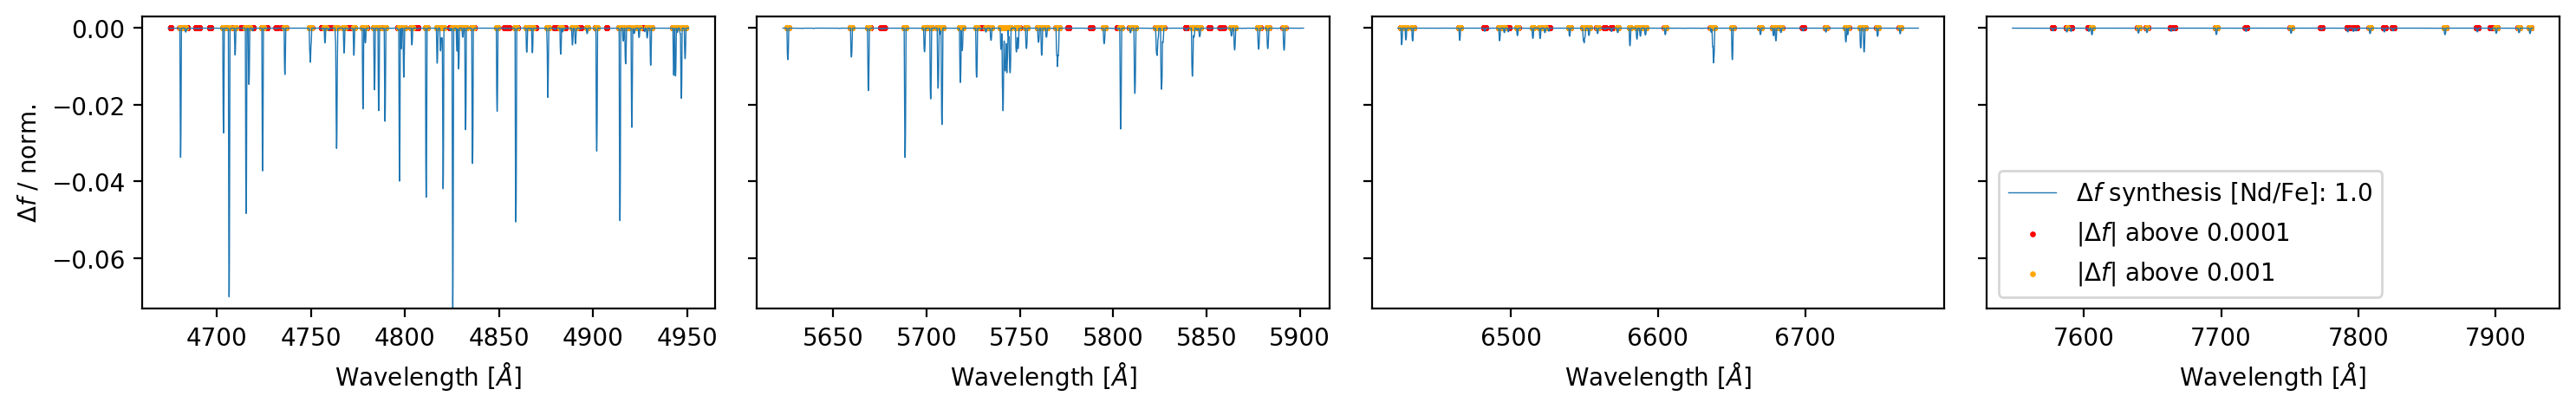
\includegraphics[width=\textwidth]{figures/gradient_spectrum_1931_nd_fe.png}
 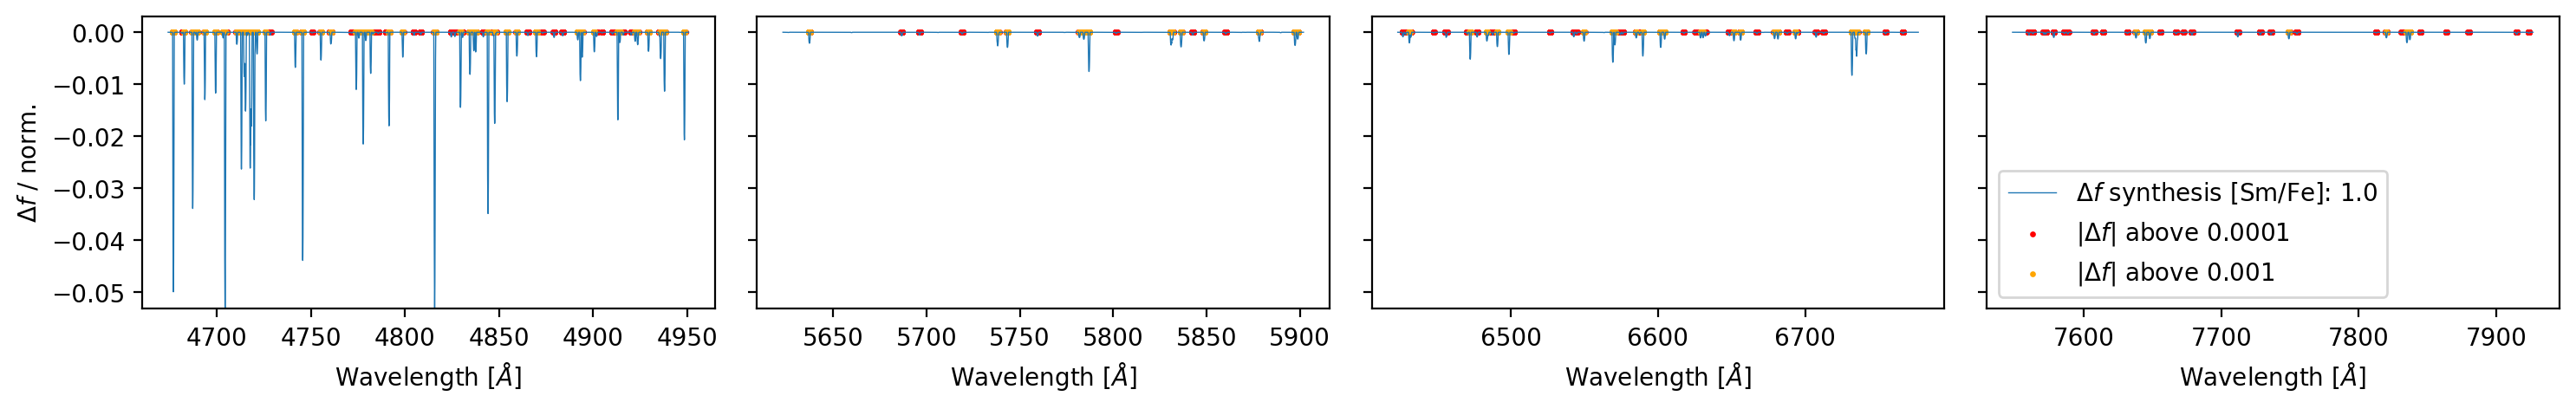
\includegraphics[width=\textwidth]{figures/gradient_spectrum_1931_sm_fe.png}
 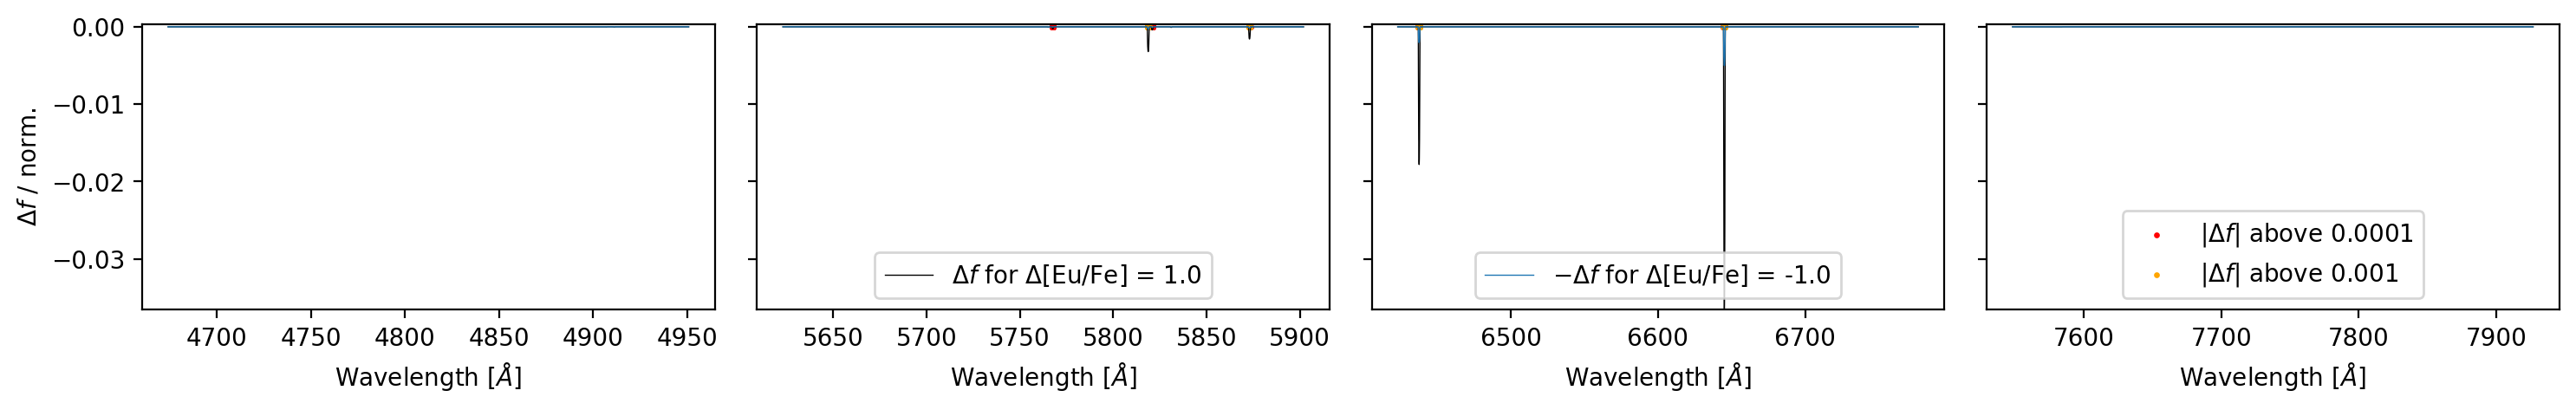
\includegraphics[width=\textwidth]{figures/gradient_spectrum_1931_eu_fe.png}
 \caption{\textbf{Continuation of Figs.~\ref{fig:gradient_spectra_1931_1}--\ref{fig:gradient_spectra_1931_4}.}} \label{fig:gradient_spectra_1931_5}
\end{figure*}

\subsection{Gradient Spectra for Arcturus-like stars}

We show the \sme gradient spectra for Arcturus-like stars in Figs.~XX--YY. These were created by a comparing rotationally broadened ($v \sin i = 24\kms$) median spectrum of the 3D bin with synthetic spectra, for which we increased (black) and decreased (blue) one particular label at a time. These were used to create masks in order to restrict \TheCannon to only those pixels, where the most extreme changes within our parameter limits caused less than \SB{0.001} change in normalised flux (orange dots).

% \section{Hospital Anxiety and Depression Scale (Italian Version)}

% \section{Openness to Discuss Cancer in the Family Scale Questionario sulla Comunicazione in Famiglia (Italian Version)}

% \begin{table}[hbt!]
% \centering
% \begin{threeparttable}
% \caption{Predicting approval of one's own house member}\label{tab:predictapproval}
% \begin{tabular}{lSSS}
%   \toprule
%   & {(1)} & {(2)} & {(3)} \\
%   \midrule
%   Religion Match & 0.077\tnote{***} & -0.029 & -0.027 \\
%                   & {(0.014)} & {(0.061)} & {(0.062)} \\
%   \bottomrule
% \end{tabular}
% \begin{tablenotes}[para]
%   \item[]Note: Entries are coefficients from a probit regression model. Robust standard errors in parentheses.
%   \item[***] $p < 0.01$,
%   \item[**] $p < 0.05$,
%   \item[*] $p < 0.1$, two-tailed test.
% \end{tablenotes}
% \end{threeparttable}
% \end{table}


\end{document}
